\documentclass[a4paper,12pt]{scrreprt}
\usepackage{scrlayer}
\DeclareNewLayer[
    foreground,
    contents={%
      \parbox[b][\layerheight][c]{\layerwidth}
        {\centering (This page intentionally left blank)}%
    }
  ]{blankpage.fg}
\DeclarePageStyleByLayers{blank}{blankpage.fg}
\usepackage{scrhack}
\usepackage{lscape}
\usepackage[utf8]{inputenc}
\usepackage[table,xcdraw]{xcolor}
\usepackage[T1]{fontenc}
\usepackage{silence}
\WarningFilter{scrreprt}{Usage of package `fancyhdr'}
\usepackage{graphicx}
\usepackage{tikz}
\usepackage{pgfplots}
\usepackage{times}
\usepackage{listings}
\usepackage{amssymb}
\usepackage{amsfonts}
\usepackage{amsmath}
\usepackage{multirow}
\usepackage[english]{babel}
\usepackage[utf8]{inputenc}
\usepackage[noend]{algpseudocode}
\usepackage[ruled,vlined,linesnumbered]{algorithm2e}
\usepackage{tabularx}
\usepackage{booktabs}
\usepackage[tikz]{mdframed}
\usepackage[toc,page]{appendix}
\usepackage{color}   %May be necessary if you want to color links
\usepackage{hyperref}
\hypersetup{
    colorlinks,
    citecolor=black,
    filecolor=black,
    linkcolor=black,
    urlcolor=black
}
\usepackage[labelfont=bf,format=plain,justification=raggedright,singlelinecheck=false]{caption}
\usepackage{mathtools}
\newenvironment{mscexample}
    {\begin{center}
    \begin{mdframed}[backgroundcolor=lightgray]}
{\end{mdframed}
    \end{center}
   }

%\algdef{SE}[DOWHILE]{Do}{doWhile}{\algorithmicdo}[1]{\algorithmicwhile\ #1}%
 
 
%\usepackage[ruled, vlined, linesnumbered, algo2e]{algorithm2e}
\DeclarePairedDelimiter\ceil{\lceil}{\rceil}
\DeclarePairedDelimiter\floor{\lfloor}{\rfloor}

\titlehead{Institut für Informatik, Universität Zürich}
\subject{\vspace*{2cm}MSc Project Report}
\title{Implementing Learned Indexes on 1 and 2 Dimensional Data}
\author{
  Neeraj Kumar, Nivedita Nivedita, Xiaozhe Yao\\[-5pt]
  %TODO: Add your matri.no and email here
  \scriptsize Matrikelnummer: 19-759-570\\[-5pt]
  \scriptsize Email: \texttt{xiaozhe.yao@uzh.ch}
}
\date{\vspace*{2cm}January 11, 2010}
\publishers{
  \small supervised by \\ 
  Prof.\ Dr.\ Michael H. Böhlen and \\ Mr. Qing\ Chen \\[5cm]
  \begin{tikzpicture}[overlay]
    \node at (-3,-3) {
\includegraphics[height=1.5cm]{IFIlogo}};
    \node at (7,-3) {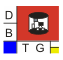
\includegraphics[height=1.5cm]{dbtgBW}};
  \end{tikzpicture}
}
 
\newtheorem{definition}{Definition}
\newtheorem{example}{Example}
\newtheorem{theorem}{Theorem}
\newtheorem{lemma}{Lemma}
\newcommand{\comment}[1]{}
\begin{document}

\begingroup
\let\newpage\relax%
\maketitle
\newpage\null\thispagestyle{blank}\newpage
\setcounter{page}{0}
\endgroup

\begin{abstract}
In this report, we 
\end{abstract}

\setcounter{tocdepth}{2}
\tableofcontents 

\chapter{Introduction}

Over the years, indexes have been widely used in databases to improve the speed of data retrieval. In the past decades, the database indexes generally fall into hand-engineered data structures and algorithms, such as B-Tree, KD-Tree, Hash Table, etc. These indexes have played an important role in databases and have been widely used in modern data management systems (DBMS). Despite their success, they do not consider the distribution of the database entries, which might be helpful in designing faster indexes.

For example, if the dataset contains integers from $1$ to $1$ million, the key can be used directly as an offset. With the key used as an offset, the values with the key can be retrieved in $\mathcal{O}(1)$ time complexity. Compared with B-Tree, which always takes $\mathcal{O}(\log n)$ time complexity for the same query. At the same time, by using the key as an offset directly, we do not need any extra overhead regarding memory space, where the B-Tree needs extra $\mathcal{O}(n)$ space complexity to save the tree.

From the above example, we found there are two promising advantages of learned indexes over hand-engineered indexes:
\begin{enumerate}
  \item Learned indexes may be faster when performing queries, especially when the number of entries in the database are extremely huge.
  \item Learned indexes may take less memory space, as we only need to save the model with constant size.
  \end{enumerate}
  
 We will explore and analyse these two advantages qualitatively in the \textit{chapter 5}. 

Nowadays, to leverage these two advantages, researchers proposed learned indexes \cite{kraska2018case}, where machine learning techniques are applied to automatically learn the distribution of the database entries and build the data-driven indexes. This approach has been shown to be powerful and competitive compared with hand-engineered indexes, such as B-Tree.

In this report, we explore the development of database indexes, from hand-engineered indexes to the learned index. After that, we explore the possibilities of using complex convolutional neural networks as database indexes. This report is organised into the following chapters:

\begin{enumerate}
	\item \textbf{Introduction}. In this chapter, we illustrate the organisation of this report. Besides, we go through the modern computer systems and introduce the general information about database indexes.
	\item \textbf{Implementation}. In this chapter, we thoroughly describe the implementation of one and two dimensional indexes, including B-Tree, baseline learned index, recursive model, KD-Tree and LISA.
	\item \textbf{Evaluation}. In this chapter, we perform evaluation among the indexes we implemented with different evaluation dataset. 
	\item \textbf{Insights and Findings}. We demonstrate our findings during the implementation in this chapter. Besides, we also discuss the advantages and disadvantages of different indexes.
	\item \textbf{Conclusions}. 
\end{enumerate}

\section{Notations}

In this report, we will use the following notations:

\begin{table}[h]
\begin{tabularx}{\textwidth}{@{}XX@{}}
\toprule
  \underline{Sets and Spaces} \\
  $\mathbb{R}$ & The set of real numbers \\
  $\mathbb{R}^d$ & The set of $d$ dimensional real space \\
  \underline{Random Variables} \\
  $\boldsymbol{X}$ & A vector or matrix \\
  $x$ & A single value in $\textbf{X}$ \\
  $(x,y)$ & A tuple contains two values \\	
  \underline{Hyper-Parameters} \\
  N   & A pre-set hyper parameter \\
  \underline{Functions} \\
  $\mathcal{LR}$ & Linear Regression Function\\
  $\mathcal{P}$ & Polynomial Function\\
  $\mathcal{M}$ & Mapping Function\\
  $\mathcal{O}$ & Big-O notation for complexity\\
  $\mathcal{SP}$ & Shard Prediction Function\\
  $\mathcal{Q}$ & Range Query \\
  $\mathcal{K}$ & $K$NN Query \\
  \underline{Others} \\
  $\clubsuit$ & End of Example \\
  $\blacksquare$ & End of Proof \\
\bottomrule
\end{tabularx}
\end{table}


\section{Terminologies}

In the following chapters, we will use the following terminologies

\textbf{Index model} is a function that maps the index of a row of data into the location (e.g. page index) of the data. For example, in one-dimensional case, the index models include B-Tree, Linear Regression models, etc.

\textbf{Key} is a special attribute in the database that could identify a record. In our work, the key could be a scalar in one-dimensional case, or a $(x,y)$ pair in two-dimensional case.

\textbf{Order of a tree} is the maximum number of children that a node can have.

\textbf{Internal node} is any node of a tree that has child nodes and is not a root node.

\textbf{Leaf node} is any node that does not have child nodes.

\textbf{Level} of a node is defined as the number of edges between this node and the root node.


\section{Motivation}

In traditional database indexes, the complexity for locating an item is usually bounded by some function related to the total number of elements. For example, with a B-Tree, an item can be found within $\mathcal{O}(\log n)$ time complexity. In the meantime, saving a B-Tree as index takes $n$ space complexity. With the rapid growing of the volume of data, $n$ becomes much larger than ever before. Hence, the big data era is calling for a database index that have constant complexity in both time and space.

To achieve such a goal, the distribution of the data is important. For example, assume that the data is fixed-length records over a set of continuous integers from 1 to 100 million, the conventional B-Tree index can be replaced by the keys themselves, making the query time complexity an $\mathcal{O}(1)$ rather than $\mathcal{O}(\log n)$. Similarly, the space complexity would be reduced from $\mathcal{O}(n)$ to $\mathcal{O}(1)$. This example shows that with the knowledge of the distribution of the data, it is possible to locate the item in database in constant time.

Formally, we define the index of each record as $x$ and the corresponding location as $y$ and we represent the whole data as $(X, Y)$ pairs with the total number of pairs defined as $N$. We could then normalise the $Y$ into $\tilde{Y}\in[0,1]$ so that the $\tilde{y}$ represents the portion of the $y$ among the whole $Y$. With these definitions, we can then define a function $F:X\to \tilde{Y}$ that maps the index into the portion of the $y$. We have $y=F(x)* N$. As the output of this function can be considered as the probability of $X\leq x$, we can regard this function $F(x)$ as the cumulative distribution function (CDF) of $X$, i.e. $F(x)=\mathbb{P}(X\leq x)$. Now that $N$ is determined by the length of data records, we only need to learn such CDF and we called the learned CDF function as \textbf{learned index model}.

From the perspective of the distribution of data records, our previous example can be rephrased as following. Our data records are $(X, Y)$ pairs with a linear relation, i.e. $y=x, \forall y\in Y$. We are looking for a function $F$ such that $y=x=F(x)* N$, and hence we end up with $F(x)=\frac{1}{N}*x$. If we use this linear function $F(x)$ as the index model, then we could locate the data within $\mathcal{O}(1)$ time complexity and we only need to store the total number of records as the only parameter. Compared with B-Tree and other indexes, the advantages are enormous.

Even though there might be potential advantages, the learned index model has several assumptions, as listed below.
\begin{enumerate}
	\item All data records are stored in memory. 
	\item All data records are sorted by $X$.
	\item All data records are stored statically in database, hence we do not take insertion and deletion into consideration.
\end{enumerate}




\chapter{Implementation}

\section{One Dimensional Data}

\subsection{B-Tree}

B-tree and its variants have been widely used as indexes in databases. B-trees can be considered as a generalisation of binary search tree: In binary search tree, there is only one key and two children at most in the internal node. B-tree extends the nodes such that each node can contain several keys and children. The keys in a node serve as dividing points and separate the range of keys. With this structure, we make a multi-way decision based on comparisons with the keys stored at the node $x$.

In this section, we introduce the construction process of B-trees and then analyse its properties.

\subsubsection{Attributes and Properties}

Each node \texttt{x} in a B-tree has the following attributes:

\begin{itemize}
\item \texttt{x.n}: the number of keys currently stored in the node $x$.
\item \texttt{x.keys}: the stored keys of this node.
\item \texttt{x.leaf}: a bool value that determines if current node is a leaf node.
\item \texttt{x.children}: a list of its children. If \texttt{x} is a leaf node who has no children at all, then the list will be empty. We assume the children are \texttt{x.$c_1$,$\cdots$,x.$c_{x.n+1}$}, i.e. there will be $\texttt{x.n}+1$ children at most.
\end{itemize}

\noindent
With these attributes, a B-tree has the following properties:

\begin{itemize}
\item The number of children of a node is always $1$ bigger than the number of keys in a node.
\item Nodes in this tree have lower and upper bounds on the number of keys they can contain. These two bounds can be expressed in terms of a fixed integer $t$, which we call the \textbf{minimum degree} of this tree.
	\begin{enumerate}
		\item Each node, other than the root node, must contain at least $t-1$ keys. The root of the tree must have at least one key if the tree is not empty.
		\item Each node can contain at most $2t-1$ keys. A node is called \textbf{full} if it contains exactly $2t-1$ keys.
	\end{enumerate}
\item Inside each node, the keys are sorted in the non-decreasing order, so that we have \texttt{x.keys$_1\leq $} \texttt{x.keys$_2\leq \cdots \leq$} \texttt{x.keys$_{\texttt{x.n}}$}.
\item The keys \texttt{x.key$_i$} separate the ranges of keys stored in each subtree: if $k_i$ is any key stored in the subtree with a root \texttt{x.c$_i$}, then we have $k_1\leq$\texttt{x.keys$_1\leq $}$ k_2\leq$\texttt{x.keys$_2\leq $} $\cdots\leq$ \texttt{x.keys$_n\leq $}$k_{\texttt{x.n}+1}$.
\end{itemize}

In Fig. \ref{fig: B-tree}, we demonstrate an example B-tree whose minimum degree is $2$. In the following section, we will illustrate how to construct and insert keys into a B-tree.

\begin{figure}
\centering
B-tree and its variants have been widely used as indexes in databases. B-trees can be considered as a generalisation of binary search tree: In binary search tree, there is only one key and two children at most in the internal node. B-tree extends the nodes such that each node can contain several keys and children. The keys in a node serve as dividing points and separate the range of keys. With this structure, we make a multi-way decision based on comparisons with the keys stored at the node $x$.

In this section, we introduce the construction process of B-trees and then analyse its properties.

\subsubsection{Attributes and Properties}

Each node \texttt{x} in a B-tree has the following attributes:

\begin{itemize}
\item \texttt{x.n}: the number of keys currently stored in the node $x$.
\item \texttt{x.keys}: the stored keys of this node.
\item \texttt{x.leaf}: a bool value that determines if current node is a leaf node.
\item \texttt{x.children}: a list of its children. If \texttt{x} is a leaf node who has no children at all, then the list will be empty. We assume the children are \texttt{x.$c_1$,$\cdots$,x.$c_{x.n+1}$}, i.e. there will be $\texttt{x.n}+1$ children at most.
\end{itemize}

\noindent
With these attributes, a B-tree has the following properties:

\begin{itemize}
\item The number of children of a node is always $1$ bigger than the number of keys in a node.
\item Nodes in this tree have lower and upper bounds on the number of keys they can contain. These two bounds can be expressed in terms of a fixed integer $t$, which we call the \textbf{minimum degree} of this tree.
	\begin{enumerate}
		\item Each node, other than the root node, must contain at least $t-1$ keys. The root of the tree must have at least one key if the tree is not empty.
		\item Each node can contain at most $2t-1$ keys. A node is called \textbf{full} if it contains exactly $2t-1$ keys.
	\end{enumerate}
\item Inside each node, the keys are sorted in the non-decreasing order, so that we have \texttt{x.keys$_1\leq $} \texttt{x.keys$_2\leq \cdots \leq$} \texttt{x.keys$_{\texttt{x.n}}$}.
\item The keys \texttt{x.key$_i$} separate the ranges of keys stored in each subtree: if $k_i$ is any key stored in the subtree with a root \texttt{x.c$_i$}, then we have $k_1\leq$\texttt{x.keys$_1\leq $}$ k_2\leq$\texttt{x.keys$_2\leq $} $\cdots\leq$ \texttt{x.keys$_n\leq $}$k_{\texttt{x.n}+1}$.
\end{itemize}

In Fig. \ref{fig: B-tree}, we demonstrate an example B-tree whose minimum degree is $2$. In the following section, we will illustrate how to construct and insert keys into a B-tree.

\begin{figure}
\centering
B-tree and its variants have been widely used as indexes in databases. B-trees can be considered as a generalisation of binary search tree: In binary search tree, there is only one key and two children at most in the internal node. B-tree extends the nodes such that each node can contain several keys and children. The keys in a node serve as dividing points and separate the range of keys. With this structure, we make a multi-way decision based on comparisons with the keys stored at the node $x$.

In this section, we introduce the construction process of B-trees and then analyse its properties.

\subsubsection{Attributes and Properties}

Each node \texttt{x} in a B-tree has the following attributes:

\begin{itemize}
\item \texttt{x.n}: the number of keys currently stored in the node $x$.
\item \texttt{x.keys}: the stored keys of this node.
\item \texttt{x.leaf}: a bool value that determines if current node is a leaf node.
\item \texttt{x.children}: a list of its children. If \texttt{x} is a leaf node who has no children at all, then the list will be empty. We assume the children are \texttt{x.$c_1$,$\cdots$,x.$c_{x.n+1}$}, i.e. there will be $\texttt{x.n}+1$ children at most.
\end{itemize}

\noindent
With these attributes, a B-tree has the following properties:

\begin{itemize}
\item The number of children of a node is always $1$ bigger than the number of keys in a node.
\item Nodes in this tree have lower and upper bounds on the number of keys they can contain. These two bounds can be expressed in terms of a fixed integer $t$, which we call the \textbf{minimum degree} of this tree.
	\begin{enumerate}
		\item Each node, other than the root node, must contain at least $t-1$ keys. The root of the tree must have at least one key if the tree is not empty.
		\item Each node can contain at most $2t-1$ keys. A node is called \textbf{full} if it contains exactly $2t-1$ keys.
	\end{enumerate}
\item Inside each node, the keys are sorted in the non-decreasing order, so that we have \texttt{x.keys$_1\leq $} \texttt{x.keys$_2\leq \cdots \leq$} \texttt{x.keys$_{\texttt{x.n}}$}.
\item The keys \texttt{x.key$_i$} separate the ranges of keys stored in each subtree: if $k_i$ is any key stored in the subtree with a root \texttt{x.c$_i$}, then we have $k_1\leq$\texttt{x.keys$_1\leq $}$ k_2\leq$\texttt{x.keys$_2\leq $} $\cdots\leq$ \texttt{x.keys$_n\leq $}$k_{\texttt{x.n}+1}$.
\end{itemize}

In Fig. \ref{fig: B-tree}, we demonstrate an example B-tree whose minimum degree is $2$. In the following section, we will illustrate how to construct and insert keys into a B-tree.

\begin{figure}
\centering
\input{graphs/implementation/one-dim/b-tree}
\caption{An example of B-tree with the minimum degree $t=2$.}
\label{fig: B-tree}
\end{figure}

\subsubsection{Insertion in a B-tree}

With a B-tree, we cannot simply create a new leaf node and insert the new key as we do with a binary search tree, because the resulting tree will fail to be a valid B-tree. Instead, we need to insert the new key into an existing leaf node. If the node is not full, we can safely insert the new key. Otherwise, we will need to split the node around the median of its keys into two new nodes and promote the median key into its parent. In this process, we need to split the parent if its parent is also full.

In the insertion, we travel down the tree and search for the position where the key should be inserted. During the traverse, we split each full node along the way. By doing so, whenever we want to split a full node, we are assured that its parent is not full. The overall algorithm is shown in Algo. \ref{algo:b-tree-insertion}, which contains methods \texttt{splitChild} and \texttt{InsertNonFull} as described in Algo. \ref{algo:b-tree-split-child} and Algo. \ref{algo:b-tree-insert-nonfull} respectively.

\begin{algorithm}[H]
\SetAlgoLined
\SetKwInOut{Input}{input}
\Input{\texttt{T}: The tree with the root \texttt{T.root}; \texttt{k}: The key to be inserted}
\KwResult{\texttt{T}: The tree with the inserted key \texttt{k}}
	\texttt{r=T.root} \\
 \uIf{\texttt{T.n==2t-1}} {
  \texttt{s = NewNode()} \\
  \texttt{T.root = s} \\
  \texttt{s.leaf = False} \\
  \texttt{s.n = 0} \\
  \texttt{s.c$_1$ = r} \\
  \texttt{SplitChild(s, 1)} \\
  \texttt{InsertNonFull(s, k)} \\
 }\uElse{
   \texttt{InsertNonFull(r, k)}
  }
 \caption{Insert}
 \label{algo:b-tree-insertion}
\end{algorithm}

In the Algo. \ref{algo:b-tree-insertion}, we first check if the root node \texttt{r} is full. If it is full, then the root splits and a new node \texttt{s} becomes the root. Then we insert the key \texttt{k} into the tree rooted at the non-full root node, i.e. \texttt{s} or \texttt{r}.

In the Algo. \ref{algo:b-tree-split-child}, the node \texttt{y} originally has $2t$ children (i.e. $2t-1$ keys) and is full. We take the following steps to split it:

\begin{enumerate}
	\item We first (from Line $1$ to Line $11$) create a new node \texttt{z} and give it the largest $t-1$ keys and the corresponding $t$ children of \texttt{y}.
	\item Then we adjust the count of keys for \texttt{y} on Line $12$: after the split, \texttt{y} will have $t-1$ keys.
	\item After that, from Line $13$ to Line $21$, we insert \texttt{z} as a child of \texttt{x}, move the median key from \texttt{y} up to \texttt{x}, and adjust the key count in \texttt{x}.
\end{enumerate}

\begin{algorithm}[H]
\SetAlgoLined
\SetKwInOut{Input}{input}
\Input{\texttt{x}: The node whose children are being split; \texttt{i}: The index of \texttt{x}'s child who is full originally}
\KwResult{\texttt{x}: The parent node whose children are not full}
\texttt{z = NewNode()} \\
\texttt{y = x.c$_i$}  \\
\texttt{z.leaf = y.leaf} \\
\texttt{z.n = t-1}\\
\For{$j\gets1$ \KwTo $t-1$}{
  \texttt{z.keys$_j$ = y.keys$_{j+t}$}\\
}
\uIf{not \texttt{y.leaf}} {
	\For{$j\gets 1$\KwTo $t$} {
		\texttt{z.c$_j$ = y.c$_{j+t}$} \\
	}
}
\texttt{y.n = t-1}\\
\For{$j\gets \texttt{x.n}$ \KwTo $i+1$} {
	\texttt{x.c$_{j+1}$ = x.c$_j$}
}
\texttt{x.c$_{i+1}$ = z} \\
\For{$j\gets \texttt{x.n}$ \KwTo $i$} {
	\texttt{x.keys$_{j+1}$=x.keys$_j$}
}
\texttt{x.key$_i$ = y.key$_t$}\\
\texttt{x.n = x.n+1}
\caption{SplitChild}
\label{algo:b-tree-split-child}	
\end{algorithm}

The Algo. \ref{algo:b-tree-insert-nonfull} works as follows:

\begin{enumerate}
	\item From Line $3$ to Line $6$, We first check if \texttt{x} is a leaf. If it is a leaf, then we insert the key \texttt{k} into \texttt{x}.
	\item If \texttt{x} is not a leaf, then we must insert \texttt{k} into the appropriate leaf node in the subtree rooted at internal node \texttt{x}. From Line $8$ to Line $11$, we traverse the subtree rooted at \texttt{x} and determine the child of \texttt{x} to which the recursion descends. Then we check on Line $12$ if the child where the recursion descends is a full node.
	\item If the child is a full node, we then split the child on Line $13$ into two non-full children. We then determine from Line $14$ to Line $15$ which of the two children is the appropriate node to insert.
	\item At the last, on Line $16$ we look into the $i$th children of \texttt{x} and recursively insert the key \texttt{k} into it.
\end{enumerate}

\begin{algorithm}[H]
\SetAlgoLined
\SetKwInOut{Input}{input}
\Input{\texttt{x}: The node to be inserted; \texttt{k}: The key to be inserted}
\KwResult{\texttt{x}: The node with the inserted key \texttt{k}}
\texttt{i=x.n} \\
\uIf{\texttt{x.leaf}} {
	\While{\texttt{i $\geq$ 1 and k < x.keys$_i$}} {
		\texttt{x.key$_{i+1}$=k} \\
		\texttt{x.n = x.n+1} \\
	}
}
\uElse{
	\While{\texttt{i $\geq$ 1 and k < x.keys$_i$}} {
		\texttt{i=i-1}\\
	}
	\texttt{i=i+1} \\
	\uIf{\texttt{x.c$_i$.n==2t-1}} {
		\texttt{SplitChild(x,i)} \\
		\uIf{\texttt{k>x.key$_i$}} {
			\texttt{i=i+1} \\
		}
	}
	\texttt{InsertNonFull(x.c$_i$, k)}
}
\caption{InsertNonFull}
\label{algo:b-tree-insert-nonfull}	
\end{algorithm}

\caption{An example of B-tree with the minimum degree $t=2$.}
\label{fig: B-tree}
\end{figure}

\subsubsection{Insertion in a B-tree}

With a B-tree, we cannot simply create a new leaf node and insert the new key as we do with a binary search tree, because the resulting tree will fail to be a valid B-tree. Instead, we need to insert the new key into an existing leaf node. If the node is not full, we can safely insert the new key. Otherwise, we will need to split the node around the median of its keys into two new nodes and promote the median key into its parent. In this process, we need to split the parent if its parent is also full.

In the insertion, we travel down the tree and search for the position where the key should be inserted. During the traverse, we split each full node along the way. By doing so, whenever we want to split a full node, we are assured that its parent is not full. The overall algorithm is shown in Algo. \ref{algo:b-tree-insertion}, which contains methods \texttt{splitChild} and \texttt{InsertNonFull} as described in Algo. \ref{algo:b-tree-split-child} and Algo. \ref{algo:b-tree-insert-nonfull} respectively.

\begin{algorithm}[H]
\SetAlgoLined
\SetKwInOut{Input}{input}
\Input{\texttt{T}: The tree with the root \texttt{T.root}; \texttt{k}: The key to be inserted}
\KwResult{\texttt{T}: The tree with the inserted key \texttt{k}}
	\texttt{r=T.root} \\
 \uIf{\texttt{T.n==2t-1}} {
  \texttt{s = NewNode()} \\
  \texttt{T.root = s} \\
  \texttt{s.leaf = False} \\
  \texttt{s.n = 0} \\
  \texttt{s.c$_1$ = r} \\
  \texttt{SplitChild(s, 1)} \\
  \texttt{InsertNonFull(s, k)} \\
 }\uElse{
   \texttt{InsertNonFull(r, k)}
  }
 \caption{Insert}
 \label{algo:b-tree-insertion}
\end{algorithm}

In the Algo. \ref{algo:b-tree-insertion}, we first check if the root node \texttt{r} is full. If it is full, then the root splits and a new node \texttt{s} becomes the root. Then we insert the key \texttt{k} into the tree rooted at the non-full root node, i.e. \texttt{s} or \texttt{r}.

In the Algo. \ref{algo:b-tree-split-child}, the node \texttt{y} originally has $2t$ children (i.e. $2t-1$ keys) and is full. We take the following steps to split it:

\begin{enumerate}
	\item We first (from Line $1$ to Line $11$) create a new node \texttt{z} and give it the largest $t-1$ keys and the corresponding $t$ children of \texttt{y}.
	\item Then we adjust the count of keys for \texttt{y} on Line $12$: after the split, \texttt{y} will have $t-1$ keys.
	\item After that, from Line $13$ to Line $21$, we insert \texttt{z} as a child of \texttt{x}, move the median key from \texttt{y} up to \texttt{x}, and adjust the key count in \texttt{x}.
\end{enumerate}

\begin{algorithm}[H]
\SetAlgoLined
\SetKwInOut{Input}{input}
\Input{\texttt{x}: The node whose children are being split; \texttt{i}: The index of \texttt{x}'s child who is full originally}
\KwResult{\texttt{x}: The parent node whose children are not full}
\texttt{z = NewNode()} \\
\texttt{y = x.c$_i$}  \\
\texttt{z.leaf = y.leaf} \\
\texttt{z.n = t-1}\\
\For{$j\gets1$ \KwTo $t-1$}{
  \texttt{z.keys$_j$ = y.keys$_{j+t}$}\\
}
\uIf{not \texttt{y.leaf}} {
	\For{$j\gets 1$\KwTo $t$} {
		\texttt{z.c$_j$ = y.c$_{j+t}$} \\
	}
}
\texttt{y.n = t-1}\\
\For{$j\gets \texttt{x.n}$ \KwTo $i+1$} {
	\texttt{x.c$_{j+1}$ = x.c$_j$}
}
\texttt{x.c$_{i+1}$ = z} \\
\For{$j\gets \texttt{x.n}$ \KwTo $i$} {
	\texttt{x.keys$_{j+1}$=x.keys$_j$}
}
\texttt{x.key$_i$ = y.key$_t$}\\
\texttt{x.n = x.n+1}
\caption{SplitChild}
\label{algo:b-tree-split-child}	
\end{algorithm}

The Algo. \ref{algo:b-tree-insert-nonfull} works as follows:

\begin{enumerate}
	\item From Line $3$ to Line $6$, We first check if \texttt{x} is a leaf. If it is a leaf, then we insert the key \texttt{k} into \texttt{x}.
	\item If \texttt{x} is not a leaf, then we must insert \texttt{k} into the appropriate leaf node in the subtree rooted at internal node \texttt{x}. From Line $8$ to Line $11$, we traverse the subtree rooted at \texttt{x} and determine the child of \texttt{x} to which the recursion descends. Then we check on Line $12$ if the child where the recursion descends is a full node.
	\item If the child is a full node, we then split the child on Line $13$ into two non-full children. We then determine from Line $14$ to Line $15$ which of the two children is the appropriate node to insert.
	\item At the last, on Line $16$ we look into the $i$th children of \texttt{x} and recursively insert the key \texttt{k} into it.
\end{enumerate}

\begin{algorithm}[H]
\SetAlgoLined
\SetKwInOut{Input}{input}
\Input{\texttt{x}: The node to be inserted; \texttt{k}: The key to be inserted}
\KwResult{\texttt{x}: The node with the inserted key \texttt{k}}
\texttt{i=x.n} \\
\uIf{\texttt{x.leaf}} {
	\While{\texttt{i $\geq$ 1 and k < x.keys$_i$}} {
		\texttt{x.key$_{i+1}$=k} \\
		\texttt{x.n = x.n+1} \\
	}
}
\uElse{
	\While{\texttt{i $\geq$ 1 and k < x.keys$_i$}} {
		\texttt{i=i-1}\\
	}
	\texttt{i=i+1} \\
	\uIf{\texttt{x.c$_i$.n==2t-1}} {
		\texttt{SplitChild(x,i)} \\
		\uIf{\texttt{k>x.key$_i$}} {
			\texttt{i=i+1} \\
		}
	}
	\texttt{InsertNonFull(x.c$_i$, k)}
}
\caption{InsertNonFull}
\label{algo:b-tree-insert-nonfull}	
\end{algorithm}

\caption{An example of B-tree with the minimum degree $t=2$.}
\label{fig: B-tree}
\end{figure}

\subsubsection{Insertion in a B-tree}

With a B-tree, we cannot simply create a new leaf node and insert the new key as we do with a binary search tree, because the resulting tree will fail to be a valid B-tree. Instead, we need to insert the new key into an existing leaf node. If the node is not full, we can safely insert the new key. Otherwise, we will need to split the node around the median of its keys into two new nodes and promote the median key into its parent. In this process, we need to split the parent if its parent is also full.

In the insertion, we travel down the tree and search for the position where the key should be inserted. During the traverse, we split each full node along the way. By doing so, whenever we want to split a full node, we are assured that its parent is not full. The overall algorithm is shown in Algo. \ref{algo:b-tree-insertion}, which contains methods \texttt{splitChild} and \texttt{InsertNonFull} as described in Algo. \ref{algo:b-tree-split-child} and Algo. \ref{algo:b-tree-insert-nonfull} respectively.

\begin{algorithm}[H]
\SetAlgoLined
\SetKwInOut{Input}{input}
\Input{\texttt{T}: The tree with the root \texttt{T.root}; \texttt{k}: The key to be inserted}
\KwResult{\texttt{T}: The tree with the inserted key \texttt{k}}
	\texttt{r=T.root} \\
 \uIf{\texttt{T.n==2t-1}} {
  \texttt{s = NewNode()} \\
  \texttt{T.root = s} \\
  \texttt{s.leaf = False} \\
  \texttt{s.n = 0} \\
  \texttt{s.c$_1$ = r} \\
  \texttt{SplitChild(s, 1)} \\
  \texttt{InsertNonFull(s, k)} \\
 }\uElse{
   \texttt{InsertNonFull(r, k)}
  }
 \caption{Insert}
 \label{algo:b-tree-insertion}
\end{algorithm}

In the Algo. \ref{algo:b-tree-insertion}, we first check if the root node \texttt{r} is full. If it is full, then the root splits and a new node \texttt{s} becomes the root. Then we insert the key \texttt{k} into the tree rooted at the non-full root node, i.e. \texttt{s} or \texttt{r}.

In the Algo. \ref{algo:b-tree-split-child}, the node \texttt{y} originally has $2t$ children (i.e. $2t-1$ keys) and is full. We take the following steps to split it:

\begin{enumerate}
	\item We first (from Line $1$ to Line $11$) create a new node \texttt{z} and give it the largest $t-1$ keys and the corresponding $t$ children of \texttt{y}.
	\item Then we adjust the count of keys for \texttt{y} on Line $12$: after the split, \texttt{y} will have $t-1$ keys.
	\item After that, from Line $13$ to Line $21$, we insert \texttt{z} as a child of \texttt{x}, move the median key from \texttt{y} up to \texttt{x}, and adjust the key count in \texttt{x}.
\end{enumerate}

\begin{algorithm}[H]
\SetAlgoLined
\SetKwInOut{Input}{input}
\Input{\texttt{x}: The node whose children are being split; \texttt{i}: The index of \texttt{x}'s child who is full originally}
\KwResult{\texttt{x}: The parent node whose children are not full}
\texttt{z = NewNode()} \\
\texttt{y = x.c$_i$}  \\
\texttt{z.leaf = y.leaf} \\
\texttt{z.n = t-1}\\
\For{$j\gets1$ \KwTo $t-1$}{
  \texttt{z.keys$_j$ = y.keys$_{j+t}$}\\
}
\uIf{not \texttt{y.leaf}} {
	\For{$j\gets 1$\KwTo $t$} {
		\texttt{z.c$_j$ = y.c$_{j+t}$} \\
	}
}
\texttt{y.n = t-1}\\
\For{$j\gets \texttt{x.n}$ \KwTo $i+1$} {
	\texttt{x.c$_{j+1}$ = x.c$_j$}
}
\texttt{x.c$_{i+1}$ = z} \\
\For{$j\gets \texttt{x.n}$ \KwTo $i$} {
	\texttt{x.keys$_{j+1}$=x.keys$_j$}
}
\texttt{x.key$_i$ = y.key$_t$}\\
\texttt{x.n = x.n+1}
\caption{SplitChild}
\label{algo:b-tree-split-child}	
\end{algorithm}

The Algo. \ref{algo:b-tree-insert-nonfull} works as follows:

\begin{enumerate}
	\item From Line $3$ to Line $6$, We first check if \texttt{x} is a leaf. If it is a leaf, then we insert the key \texttt{k} into \texttt{x}.
	\item If \texttt{x} is not a leaf, then we must insert \texttt{k} into the appropriate leaf node in the subtree rooted at internal node \texttt{x}. From Line $8$ to Line $11$, we traverse the subtree rooted at \texttt{x} and determine the child of \texttt{x} to which the recursion descends. Then we check on Line $12$ if the child where the recursion descends is a full node.
	\item If the child is a full node, we then split the child on Line $13$ into two non-full children. We then determine from Line $14$ to Line $15$ which of the two children is the appropriate node to insert.
	\item At the last, on Line $16$ we look into the $i$th children of \texttt{x} and recursively insert the key \texttt{k} into it.
\end{enumerate}

\begin{algorithm}[H]
\SetAlgoLined
\SetKwInOut{Input}{input}
\Input{\texttt{x}: The node to be inserted; \texttt{k}: The key to be inserted}
\KwResult{\texttt{x}: The node with the inserted key \texttt{k}}
\texttt{i=x.n} \\
\uIf{\texttt{x.leaf}} {
	\While{\texttt{i $\geq$ 1 and k < x.keys$_i$}} {
		\texttt{x.key$_{i+1}$=k} \\
		\texttt{x.n = x.n+1} \\
	}
}
\uElse{
	\While{\texttt{i $\geq$ 1 and k < x.keys$_i$}} {
		\texttt{i=i-1}\\
	}
	\texttt{i=i+1} \\
	\uIf{\texttt{x.c$_i$.n==2t-1}} {
		\texttt{SplitChild(x,i)} \\
		\uIf{\texttt{k>x.key$_i$}} {
			\texttt{i=i+1} \\
		}
	}
	\texttt{InsertNonFull(x.c$_i$, k)}
}
\caption{InsertNonFull}
\label{algo:b-tree-insert-nonfull}	
\end{algorithm}


\subsection{Baseline Learned Index}

\subsubsection{Overview}

The B-Tree can be regarded as a function $\mathcal{F}$ that maps the key $x$ into its corresponding page index $y$. It is known to us that the pages are allocated in a way that the every $S$ entries are allocated in a page where $S$ is a pre-defined parameter. For example, if we set $S$ to be 10 items per page, then the first page will contain the first 10 keys and their corresponding values. Similarly, the second 10 keys and their corresponding values will be allocated to the second page.

If we know the CDF of $X$ as $F(X\leq x)$ and the total number of entries $N$, then the position of $x$ can be estimated as $p=F(x)*N$ and the page index where it should be allocated to is given by

$$y=\floor{\frac{p}{S}}=\floor{\frac{F(x)*N}{S}}$$  

For example, if the keys are uniformly distributed from $0$ to $1000$, i.e. the CDF of $X$ is defined as $F(X\leq x)=\frac{x}{1000}$ and we set $S=10, N=1001$. Then for any key $x$, we immediately know it will be allocated into $y=\floor{\frac{1000}{10}*\frac{x}{1000}}=\floor{\frac{x}{10}}$. Assume that we have a key $698$, then we can calculate $y=\floor{\frac{698}{10}}=69$. By doing so, the page index is calculated in constant time and space.

In this example, we see that the distribution of $X$ is essential and our goal of learned index in one-dimensional data is to learn such distribution. To do so, we apply two different techniques as the baseline, the polynomial regression and fully connected neural network.

To train such a learned index, we first manually generate the $X$ with respect to a certain distribution. We then save the generated $X$ into a dense array with the length $N$. Then we use the proportional index, i.e. the index of each $x$ divided by $N$ as the expected output $y$.

\subsubsection{Polynomial Regression}
 
The polynomial regression model with degree $m$ can be formalised as 

$$ \hat{y_i}= \beta_0+\beta_1x_i+\beta_2x_i^2+\cdots+\beta_mx_i^m$$ and it can be expressed in a matrix form as below

$$
\begin{bmatrix}
y_1 \\ y_2\\ \vdots \\ y_n 
\end{bmatrix}=\begin{bmatrix}
1 & x_1 & x_1^2 &\cdots & x_1^m \\ 
1 & x_2 & x_2^2 &\cdots & x_2^m \\ 
\vdots \\ 
1 & x_n & x_n^2 &\cdots & x_n^m \\ 
\end{bmatrix}\begin{bmatrix}
\beta_0 \\ \beta_1 \\ \vdots \\ \beta_m 
\end{bmatrix}
$$ which can be written as $Y=\boldsymbol{X}\boldsymbol{\beta}$. 
 
 Our goal is to find $\beta$ such that the sum of squared error, i.e. $\text{S}(\boldsymbol{\beta})=\sum_{i=1}^n(\hat{y}-y)^2$ is minimal. This optimisation problem can be resolved by ordinary least square estimation as shown below.
 
 First we have the error as
 
 \begin{equation}
 \begin{split}
 \text{S}(\boldsymbol{\beta})=||\boldsymbol{y}-\boldsymbol{X} \boldsymbol{\beta}||& =(\boldsymbol{y}-\boldsymbol{X}\boldsymbol{\beta})^T(\boldsymbol{y}-\boldsymbol{X}\boldsymbol{\beta})\\
 	& =\boldsymbol{y}^T\boldsymbol{y}-\boldsymbol{\beta}^T\boldsymbol{X}^T\boldsymbol{y}-\boldsymbol{y}^T\boldsymbol{X}\boldsymbol{\beta}+\boldsymbol{\beta}^T\boldsymbol{X}^T\boldsymbol{X}\boldsymbol{\beta}
\end{split}
 \end{equation}
 
 Here we know that $(\boldsymbol{\beta}^T\boldsymbol{X}^T\boldsymbol{y})^T=\boldsymbol{y}^T\boldsymbol{X}\boldsymbol{\beta}$ is a $1\times 1$ matrix, i.e. a scalar. Hence it is equal to its own transpose. As a result we could simplify the error as
 
 \begin{equation}
 	\begin{split}
 		\text{S}(\boldsymbol{\beta})=\boldsymbol{y}^T\boldsymbol{y}-2\boldsymbol{\beta}^T\boldsymbol{X}^T\boldsymbol{y}+\boldsymbol{\beta}^T\boldsymbol{X}^T\boldsymbol{X}\boldsymbol{\beta}
 	\end{split}
 \end{equation}
 
 In order to find the minimum of $S(\boldsymbol{\beta})$, we differentiate it with respect to $\boldsymbol{\beta}$ as 
 
 \begin{equation}
 	\nabla_{\boldsymbol{\beta}}S=-2\boldsymbol{X}^T\boldsymbol{y}+2(\boldsymbol{X}^T\boldsymbol{X})\boldsymbol{\beta}
 \end{equation}
 
 By let it to be zero, we end up with 
 
 \begin{equation}
 \begin{split}
 	 &	-\boldsymbol{X}^T\boldsymbol{y}+(\boldsymbol{X}^T\boldsymbol{X})\boldsymbol{\beta}=0 \\
 	& \implies \boldsymbol{\beta}= (\boldsymbol{X}^T\boldsymbol{X})^{-1}\boldsymbol{X}^T\boldsymbol{y}
 \end{split}
 \end{equation}
 
\subsubsection{Fully Connected Neural Network}

\subsection{Recursive Model Index}

%TODO: there should be some graph to demonstrate the last-mile problem.

In our baseline models, it is not very difficult to reduce the mean square error from millions to thousands. However, it is much harder to reduce it from thousands to tens. This is the so called last-mile problem.

In order to solve this problem, recursive model index was proposed \cite{kraska2018case}. The idea is to split the whole set of data into smaller pieces and assign each piece an index model. By doing so, each model is only responsible for a small range of keys. Ideally, in each smaller range, the keys are distributed in a way that is easier to be learned by our index models, such as polynomial model, fully connected model or even traditional B-Tree model.

As shown in Fig. \ref{rmi_structure}. A recursive model can be regarded as a tree structure, which contains a root model that receives the full dataset for training. Then the root model will split the dataset into several parts. Each sub-model will then receive one part of the full dataset. Then we train the sub-models one by one with the partial training dataset. 

\begin{mscexample}
	For example, in the Fig. \ref{rmi_structure}, the full dataset will be split into three parts and each sub-model receives one part. To train this recursive model, we first train the root model with the whole dataset. Then the root model will split the dataset into 3 parts according to the predicted value of each data point in the dataset. Then each sub-model will receive one part and we train the sub-model accordingly.
\end{mscexample}

\begin{figure*}[h]
\centering
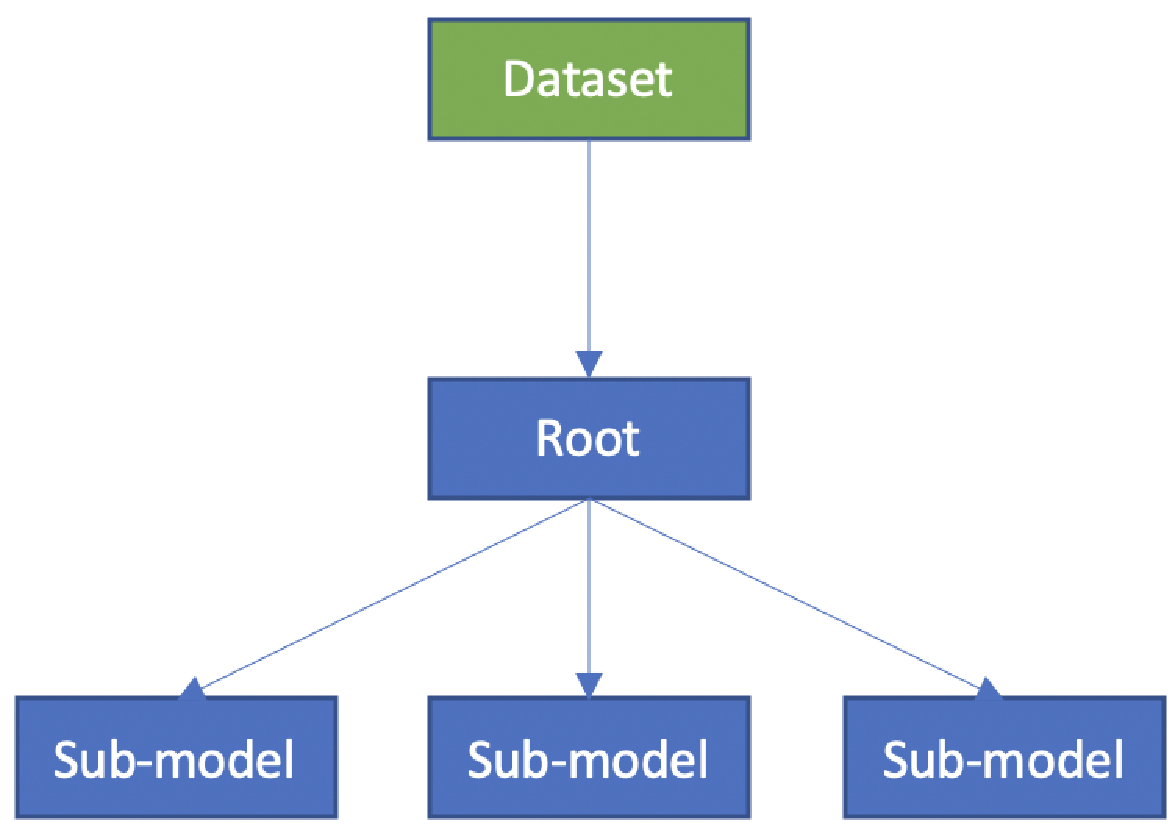
\includegraphics[scale=0.4]{graphs/rmi_demo}
\caption{An example recursive model index with one root model and three leaf model.}
\label{rmi_structure}
\end{figure*}



\subsubsection{Definitions}

Similar to a tree, we define the following terms in a recursive model:

\begin{enumerate}
	\item \textbf{Node Model}. Every node is responsible for making decisions with given input data. In one dimensional case, it can be regarded as a function $f:\mathbb{R}\to\mathbb{R}, x\to y$ where $x$ is the input index and $y$ is the corresponding page block. In principle, each node can be implemented as any machine learning model, from linear regression to neural network, or a traditional tree-based model, such as B-Tree.
	\item \textbf{Internal Node Model}. Internal nodes are all nodes except for leaf nodes and the root node. Every internal node receives a certain part of training data from the full dataset, and train a model on it. 
\end{enumerate}

In the following sections, we will use the notations defined below:
\begin{enumerate}
	\item $N_M^{(i)}$ is the number of models in the $i$th stage.
	%TODO: more notations
	%TODO: modify algorithms accordingly
\end{enumerate}


\subsubsection{Training}

In order to construct a recursive model, we need to have several parameters listed below:
\begin{enumerate}
	\item The training dataset, notated as $(X, Y)$ with entries notated as $(x,y)$.
	\item The number of stages, notated as $N_S$. It is an integer variable.
	\item The number of models at each stage, notated as $N_M$. It is a list of integer variable. $N_M^{(i+1)}$ represents the number of models in the $i$th stage.
\end{enumerate}

The training process of recursive model is an up-bottom process. There will be only one root model that receives the whole training data. After the root model is trained, we iterate over all the training data and predict the page by the root model. After the iteration, we get a new set of pairs $(X, Y_0)$. Then we map $\forall y_0\in Y_0$ into the selected model id in next stage by $\texttt{next}=y_0 * N_M^{(i+1)}/\texttt{max(Y)}$.

\begin{algorithm}[H]
    \SetAlgoLined
    \SetKwInOut{Input}{input}
    \Input{\texttt{num\_of\_stages; num\_of\_models; types\_of\_models; x; y}}
     \texttt{trainset=[[(x,y)]]} \\
     \texttt{stage$\gets 0$} \\
     \While{\texttt{stage} \textless \texttt{num\_of\_stages}}{
      \While{\texttt{model} \textless \texttt{num\_of\_models[stage]}} {
        \texttt{model.train(trainset[stage][model])} \\
        \texttt{models[stage].append(model)}
      }
      \uIf{not last stage} {
        \For{$i\gets0$ \KwTo $len(x)$}{
            	\texttt{model=models[output from previous stage]} \\
            	\texttt{output=model.predict(x[i])} \\
            	\texttt{next=output * num\_of\_models[stage+1]/max\_y} \\
            	\texttt{trainset[stage+1][next].add((x[i],y[i]))}
        }
      }
     }
     \caption{Training of Recursive Model Index}
\end{algorithm}

\subsubsection{Prediction}

\begin{algorithm}[H]
    \SetAlgoLined
    \SetKwInOut{Input}{input}
    \Input{\texttt{x; models; num\_of\_stages; max\_y}}
     \texttt{stage$\gets 0$} \\
 	 \texttt{next\_model$\gets 0$} \\
     \While{\texttt{stage} \textless \texttt{num\_of\_stages}}{
        \texttt{output = model.predict(x)} \\
        \texttt{next\_model=output*len(models[stage+1])/max\_y}\\ 
      \uIf{last stage} {
		\texttt{y = next}
      }
     }
     \caption{Training of Recursive Model Index}
\end{algorithm}

\subsubsection{Polynomial Internal Models}

In the recursive model index, we use internal models to learn the CDF of a part of the full training data. In order to learn the CDF, we need to know or assume the distribution of a specific part of the data. In this report, we support the following distributions.

\begin{table}[h]
  \begin{tabularx}{\textwidth}{@{}XX@{}}
  \toprule
    Linear Regression & $wx+b$ \\
    Quadratic Regression & $ax^2+bx+c$ \\
    B-Tree & N/A \\
    Fully Connected Neural Network & N/A \\
  \bottomrule
  \end{tabularx}
  \end{table}

Here we describe how we fit a polynomial model.

The polynomial regression model with degree $m$ can be formalised as 

$$ \hat{y_i}= \beta_0+\beta_1x_i+\beta_2x_i^2+\cdots+\beta_mx_i^m$$ and it can be expressed in a matrix form as below

$$
\begin{bmatrix}
y_1 \\ y_2\\ \vdots \\ y_n 
\end{bmatrix}=\begin{bmatrix}
1 & x_1 & x_1^2 &\cdots & x_1^m \\ 
1 & x_2 & x_2^2 &\cdots & x_2^m \\ 
\vdots \\ 
1 & x_n & x_n^2 &\cdots & x_n^m \\ 
\end{bmatrix}\begin{bmatrix}
\beta_0 \\ \beta_1 \\ \vdots \\ \beta_m 
\end{bmatrix}
$$ which can be written as $Y=\boldsymbol{X}\boldsymbol{\beta}$. 
 
 Our goal is to find $\beta$ such that the sum of squared error, i.e. $\text{S}(\boldsymbol{\beta})=\sum_{i=1}^n(\hat{y}-y)^2$ is minimal. This optimisation problem can be resolved by ordinary least square estimation as shown below.
 
 First we have the error as
 
 \begin{equation}
 \begin{split}
 \text{S}(\boldsymbol{\beta})=||\boldsymbol{y}-\boldsymbol{X} \boldsymbol{\beta}||& =(\boldsymbol{y}-\boldsymbol{X}\boldsymbol{\beta})^T(\boldsymbol{y}-\boldsymbol{X}\boldsymbol{\beta})\\
 	& =\boldsymbol{y}^T\boldsymbol{y}-\boldsymbol{\beta}^T\boldsymbol{X}^T\boldsymbol{y}-\boldsymbol{y}^T\boldsymbol{X}\boldsymbol{\beta}+\boldsymbol{\beta}^T\boldsymbol{X}^T\boldsymbol{X}\boldsymbol{\beta}
\end{split}
 \end{equation}
 
 Here we know that $(\boldsymbol{\beta}^T\boldsymbol{X}^T\boldsymbol{y})^T=\boldsymbol{y}^T\boldsymbol{X}\boldsymbol{\beta}$ is a $1\times 1$ matrix, i.e. a scalar. Hence it is equal to its own transpose. As a result we could simplify the error as
 
 \begin{equation}
 	\begin{split}
 		\text{S}(\boldsymbol{\beta})=\boldsymbol{y}^T\boldsymbol{y}-2\boldsymbol{\beta}^T\boldsymbol{X}^T\boldsymbol{y}+\boldsymbol{\beta}^T\boldsymbol{X}^T\boldsymbol{X}\boldsymbol{\beta}
 	\end{split}
 \end{equation}
 
 In order to find the minimum of $S(\boldsymbol{\beta})$, we differentiate it with respect to $\boldsymbol{\beta}$ as 
 
 \begin{equation}
 	\nabla_{\boldsymbol{\beta}}S=-2\boldsymbol{X}^T\boldsymbol{y}+2(\boldsymbol{X}^T\boldsymbol{X})\boldsymbol{\beta}
 \end{equation}
 
 By let it to be zero, we end up with 
 
 \begin{equation}
 \begin{split}
 	 &	-\boldsymbol{X}^T\boldsymbol{y}+(\boldsymbol{X}^T\boldsymbol{X})\boldsymbol{\beta}=0 \\
 	& \implies \boldsymbol{\beta}= (\boldsymbol{X}^T\boldsymbol{X})^{-1}\boldsymbol{X}^T\boldsymbol{y}
 \end{split}
 \end{equation}

  

\section{Two Dimensional Data}

\subsection{KD-Tree}

KD-Tree is a space partitioning structure which can be used to organise data points in k dimensional space. We have fixed our dimensions of data points  to 2-dimensions and their values are stored in 1-dimension. In our implementation KD-Tree is a binary tree with every node having data points partitioned in 2-dimensional space.\\\\\

\subsubsection{Definitions}

\begin{figure}[htp]
    \centering
    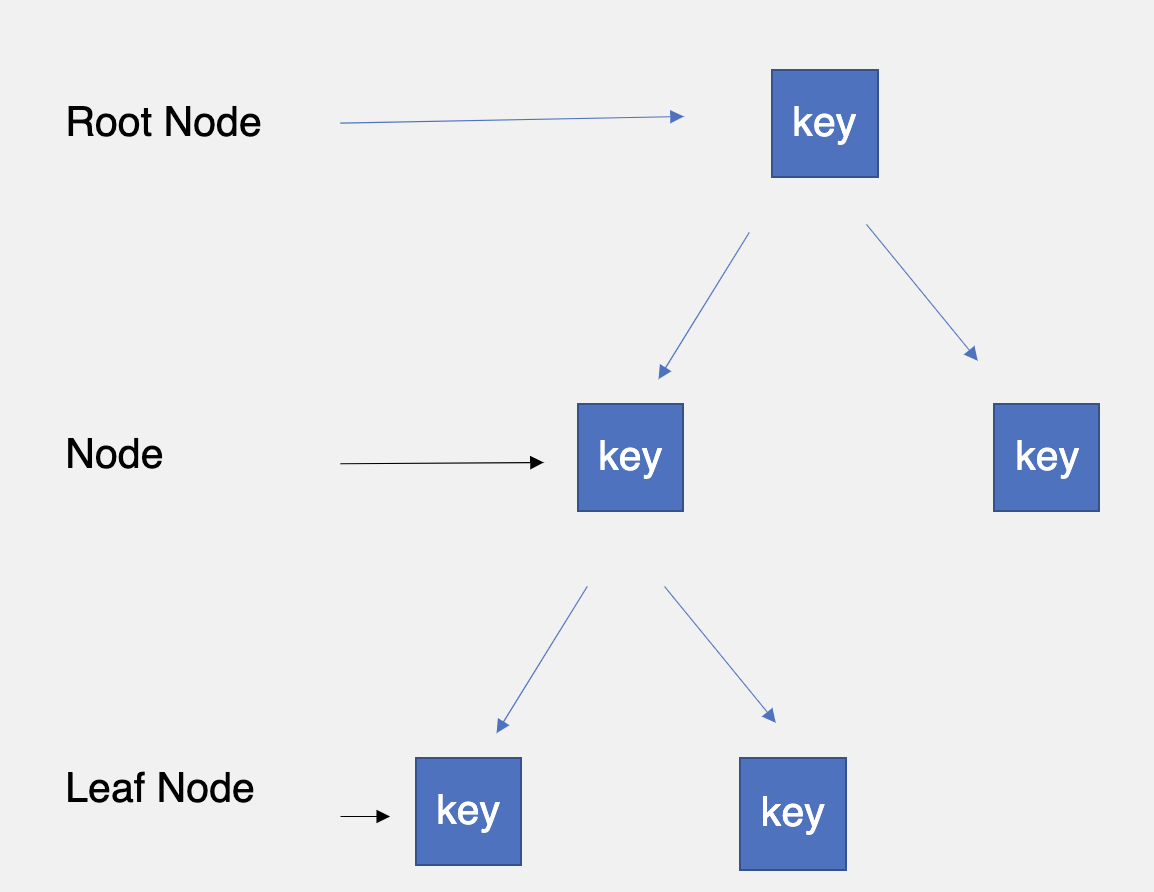
\includegraphics[width=0.6\textwidth]{graphs/KD-Tree.png}
    \caption{KD-Tree}
    \label{fig:KD-Tree}
\end{figure}

\begin{enumerate}
    \item\textbf{{Node}}: Node of a KD-Tree is essentially a 2-dimensional data point. It can be k-dimensional for KD-Tree.
    \item\textbf{{Root Node}}: Root Node is the Node with no parents and has other nodes/leaves as children. Each node can have two child nodes since it is a binary tree. 
    \item\textbf{{Leaf Node}}: Leaves of a tree are the nodes which do not have any child nodes.
    \item\textbf{{Dimensions}}: Every KD-Tree can be structured in such a way that the data points are divided into k-dimensions. Each node is recursively cut into as many dimensions as is mentioned in the dimensions. In our case the data points are 2-dimensional and hence the space is divided in 2-dimensions alternatively until a leaf is reached.\\
\end{enumerate}
    
\begin{algorithm}[H]
    \SetAlgoLined
    \SetKwInOut{Input}{Input}
    \SetKwInOut{Output}{Output}
    \Input{Point list; trainset=[$(x,y);x \in \mathbb{R}^{2};y \in \mathbb{R}$], dimension = 2, $int$ split axis; 0 or 1}
    \Output{KD-Tree}
    \For{$i\gets0$ \KwTo $len(Point list)$}{
    \texttt{$int$ split axis := split axis mod $dim$} // Select the split axis based on depth\\
    \texttt{Sort point list and choose median}\\
    \texttt{Create node at median}\\
    \texttt{node.leftChild := kdtree(points in pointList before median, split axis+1); //SubTree Creation \\ 
    node.rightChild := kdtree(points in pointList after median, split axis+1);}
     \caption{Training Algorithm for KD-Tree}
     \label{Training_KD-Tree}
     }
\end{algorithm}

For constructing the KD-Tree we have following consttraints:


\begin{enumerate}
    \item {As one moves down the tree, one cycles through the axes used to select the splitting planes. For example, in a 2-dimensional plane we split the data on x-axis at the root and then split it on y-axis for it's children. We then split the grandchildren on x-axis again and so on.}
    \item {Points are inserted by selecting the median of the points being put into the subtree, with respect to their coordinates in the axis being used to create the splitting plane. This ensures that the tree is balanced. A balanced tree is the one in which leaf node is approximately the same distance from the root.}\\
\end{enumerate}    
    
In the algorithm above, we first sort all the values obtained in the Point list. We initialise the first split axis to 0 and then toggle between 0 and 1 as we increase the depth. Once the data points are sorted, their median is chosen. For example if we have points sorted as [[3,4],[5,6],[7,8]], we will take the median as [5,6] and assign [3,4] to the left and [7,8] to the right. The reason node.leftChild = [1,2] is because 1 < 5 and node.rightChild = [7,8] is because 7 > 5 i.e., we compare the x-axis of the points to the root when we create the subsequent nodes. This process is then carried out recursively and subtrees are created on the left and right until all the points are added to the tree from the Point list.

\subsubsection{Construction time of 2-dimensional kd-tree:}

The most expensive part of the construction of KD-Tree is sorting the points on both the axis. Instead of working with more complex algorithm to find the median we first presorted the values on x-axis and then on y-axis. Hence the time complexity is $O( n log n)$. Since KD-Tree is A binary tree, and every leaf and internal node uses O(1) storage, the total storage is $O(n)$.


\subsubsection{Introduction to Range Searching}

\begin{figure}[htp]
    \centering
    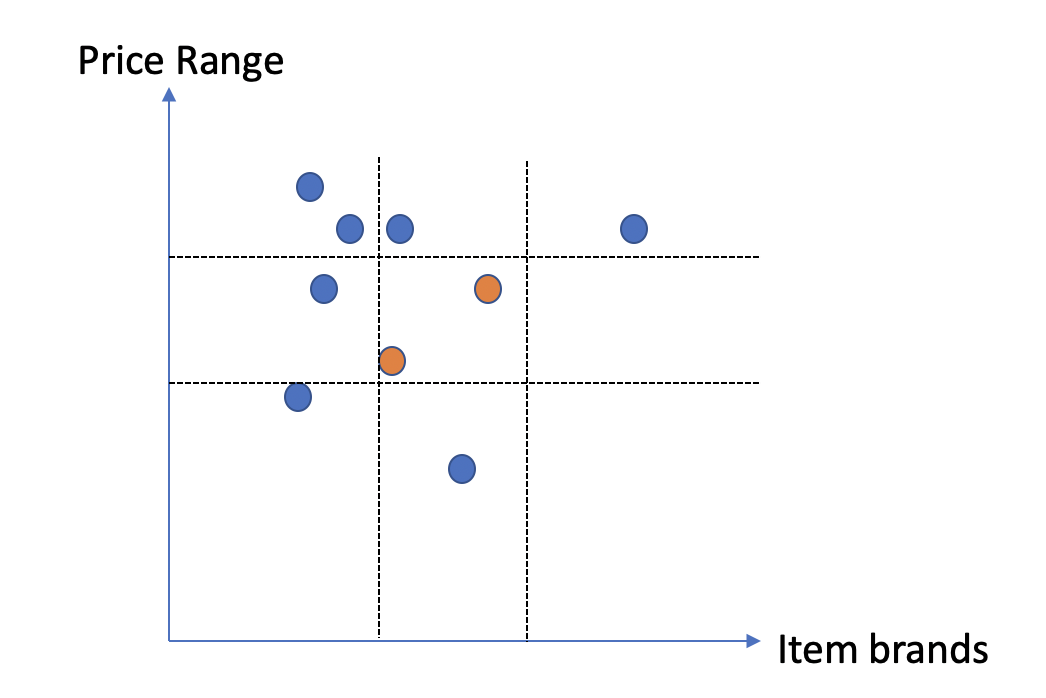
\includegraphics[width=0.6\textwidth]{graphs/Range_Query_Intro.png}
    \caption{KD-Tree Range Query}
    \label{fig:KD_ee_Range_Query_Intro}
\end{figure}

Range searching is basically to search data which lie within a specified range. For example if you have a database where you store data of a number of items and their price ranges. You want to search items from a specific brand and within a specific price range. You can search for this data by specifying these parameters. In our model we can pass the lower bound and upper bound of a rectangle and all the points that lie within those bounds are retrieved in the 2-dimensional plane.


\begin{figure}[htp]
    \centering
    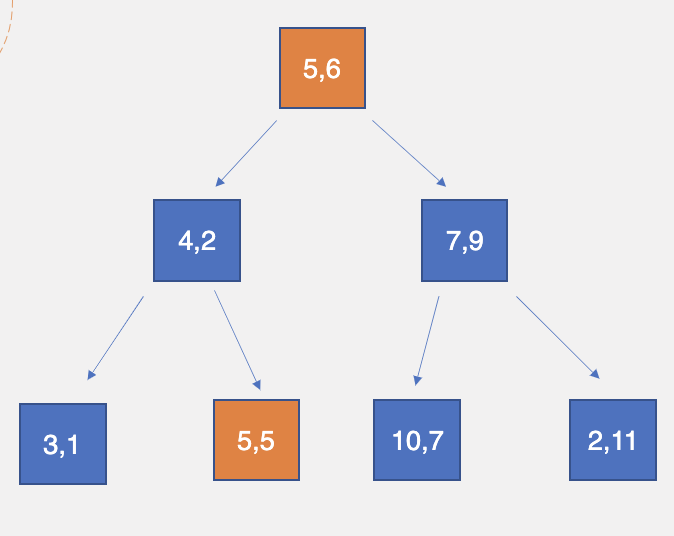
\includegraphics[width=0.6\textwidth]{graphs/Range_Query_Tree.png}
    \caption{KD-Tree for Range Query}
    \label{fig:KD-Tree_for_Range Query}
\end{figure}

\begin{figure}[htp]
    \centering
    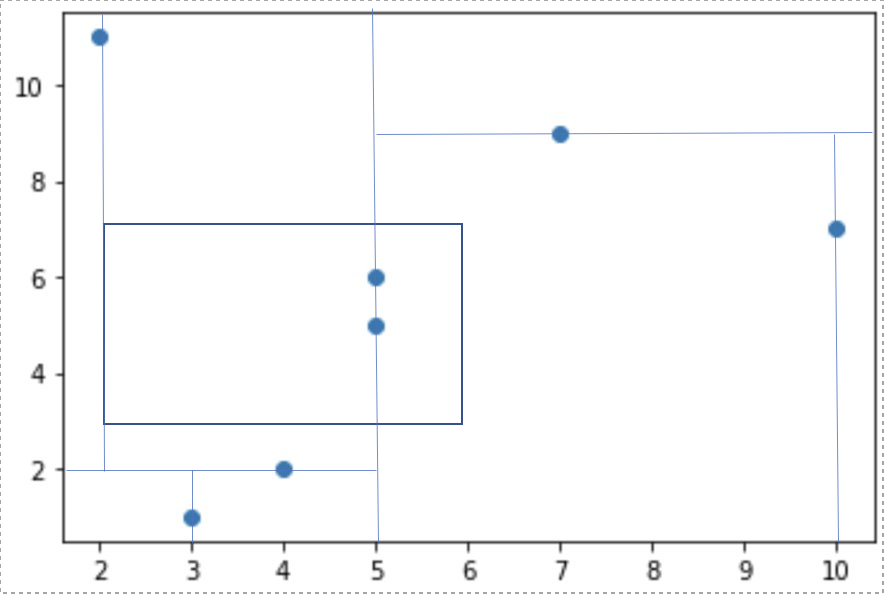
\includegraphics[width=0.6\textwidth]{graphs/Range_Query_plot.png}
    \caption{KD-Tree Range Query Plot on 2-dimentional plane}
    \label{fig:KD_Tree_Range_Query_Plot}
\end{figure}

In our model in range query we first generate lower and upper bound of the rectangle randomly. We then check if the root of the tree lies within the range of the bounds and only then start traversing the tree. For example we have a tree with Point list as 

	$$[(5,6),[4,2],[7,9],[3,1],[5,5],[10,7],[2,11]]$$
	
	and with lower bound = [2,3] and upper bound = [6,7], we will get a tree as is shown in \ref{fig:KD-Tree_for_Range Query}. We can see the points along with the rectangle range plotted in \ref{fig:KD_Tree_Range_Query_Plot}. Points [5,5] and [5,6] are returned in the query since they lie within the rectangle as seen in the plot. First the root point is checked and since the x coordinate and y coordinate both lie within the rectangle bounds i.e., 2 > 5 > 6 and 3 > 6 > 7. It then checks if the x coordinate is lower than or greater than the lower bound x coordinate. Since the value is larger than lower bound x coordinate that is 2 it will then traverse to the left. In the left it has child node as [4,2] however, since the y coordinate doesn't lie in the range of the upper bound this point is not selected. Therefore, it recursively traverses the tree and checks if the point lies within the bound until it reaches a leaf.

\subsubsection{K-nearest neighbour}

K-nearest neighbour as the name suggests is the process to find the k nearest neighbour to the test point that we are looking for. For example in a database if you have coordinates of various famous restaurants stored and you want to query 5 nearest restaurants to your current location then the query should fetch you 5 nearest restaurants depending on your current location on the map. Your current coordinate can be any value and may not be a subset of the data. \\

In our model k-nearest neighbour is calculated based on the euclidean distance of the test data point with respect to the other points. We have also compared the result of our model with standard packages of scipy sklearn to verify the results of the distance calculated and the points returned. Since measuring distance of each point from the test point is computationally very expensive we exploit the tree structure of the KD-Tree to prune the tree and only measure distance with much fewer points and only traverse a subtree if required. \\

\begin{figure}[htp]
    \centering
    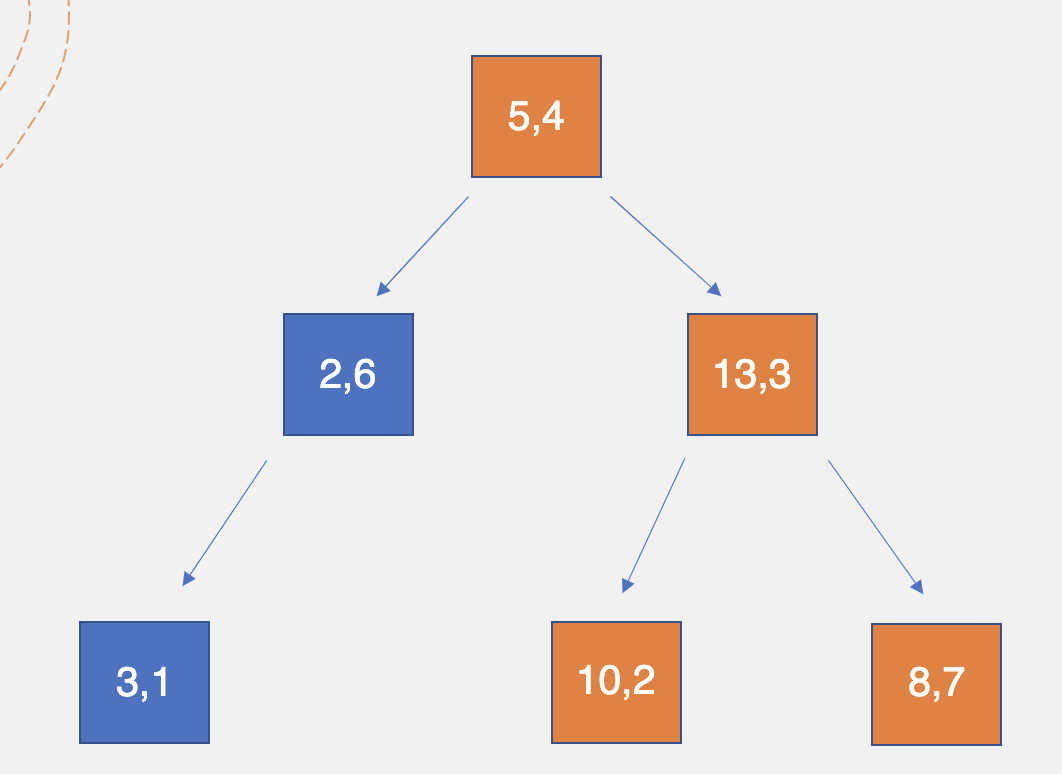
\includegraphics[width=0.6\textwidth]{graphs/KD-Tree_KNN_Tree.png}
    \caption{KD-Tree for KNN Query}
    \label{fig:KD-Tree_for_KNN Query}
\end{figure}

\begin{figure}[htp]
    \centering
    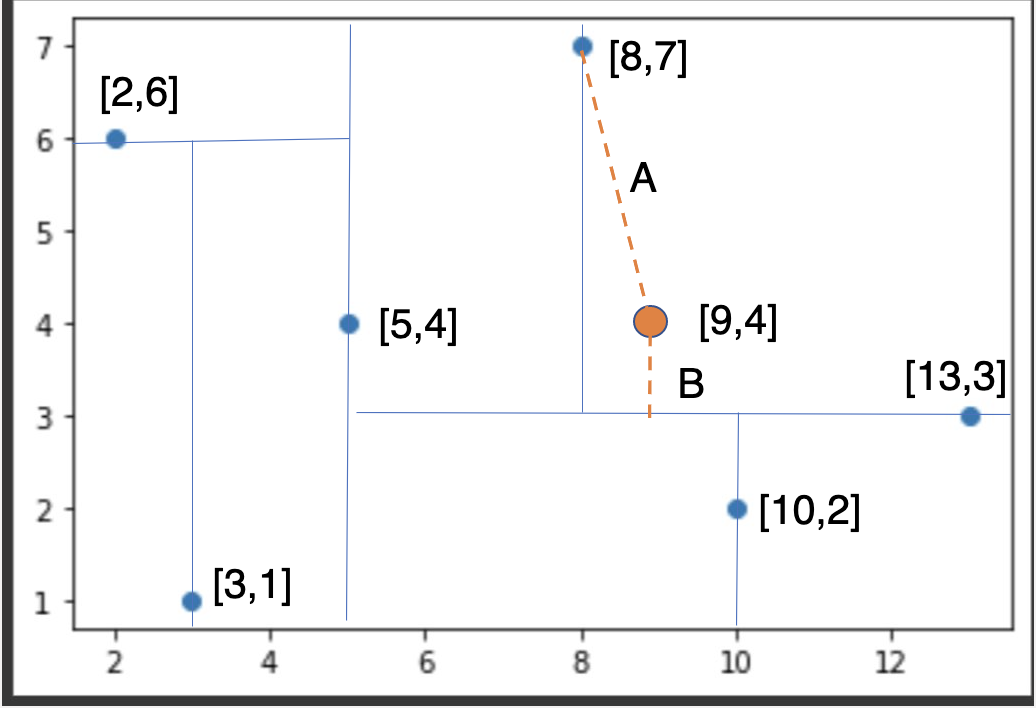
\includegraphics[width=0.6\textwidth]{graphs/KD-Tree_KNN_plot.png}
    \caption{KD-Tree KNN Plot on 2-dimentional plane}
    \label{fig:KD_Tree_KNN_Plot}
\end{figure}


\begin{mscexample}
	For example, we have Point list as $[(5,4),[2,6],[13,3],[8,7],[3,1],[10,2]]$ then we will have a tree structure as shown in \ref{fig:KD-Tree_for_KNN Query} and it's plot on 2-dimensional plane is shown in \ref{fig:KD_Tree_KNN_Plot}. As we can see in \ref{fig:KD_Tree_KNN_Plot} that even though point [8,7] is the leaf we will reach when we traverse the tree to search for point nearest to test point [9,4] it is not infact the nearest point to the test data. In this case if we want to look for 4 nearest neighbour, we first check the square of euclidean distance of [9,4] with the root of the tree i.e., [5,4] which is 16. It then calculates the distance with [2,6] and [13,3] which calculates to 53 and 17 respectively. It then keeps traversing to the right node while calculating distance until it reaches a leaf. After reaching the leaf it then checks the distance with [8,7] with a distance of 10 which is infact smaller than the previous shortest distance of 16 with the root. It adds these points to the list. It then makes a decision weather to go left from [13,3] based on the distance of the test point with leaf [8,7] i.e., A and the perpendicular distance with point [13,3] which is B. Since distance A > B as can be seen in the figure \ref{fig:KD_Tree_KNN_Plot} there is a chance that there could a point in the subtree with a distance smaller than the previous points. In this case it will then check the distance with point [10,2] and the distance is the shortest(best distance) so far of 5. 
\end{mscexample}



\subsection{LISA: Learned Index for Spatial Data}

\comm{
\subsubsection{LISA Baseline model Limitation}

Prediction cost in baseline method consists of following two parts.

\begin{enumerate}
	\item Search cost for the cell which contains the key. This cost will be equal to $log_{2}N_{1}$, where $N_{1}$ is the number of cells into which mapped values are divided.
	
	\item Cost associated with sequentially comparing the query point key value against keys inside the cell found in previous search. On average this cost will be equal to $N_{2}\slash2$, where $N_{2}$ is the number of keys in a cell.   
	
If cell size is large, number of cells will be smaller, number of keys per cell will be higher, resulting in higher cost of sequential scan with in the cell. 
\end{enumerate}
Consider the example in figure \ref{fig:BaseLine_Method_Limitation}. Dataset is divided into 3 sections based on the mapped values. Any point or range query in the second triangle(page) will result into a sequential scan through all 9 keys in the cells.

\begin{figure*}[t]
    \centering
    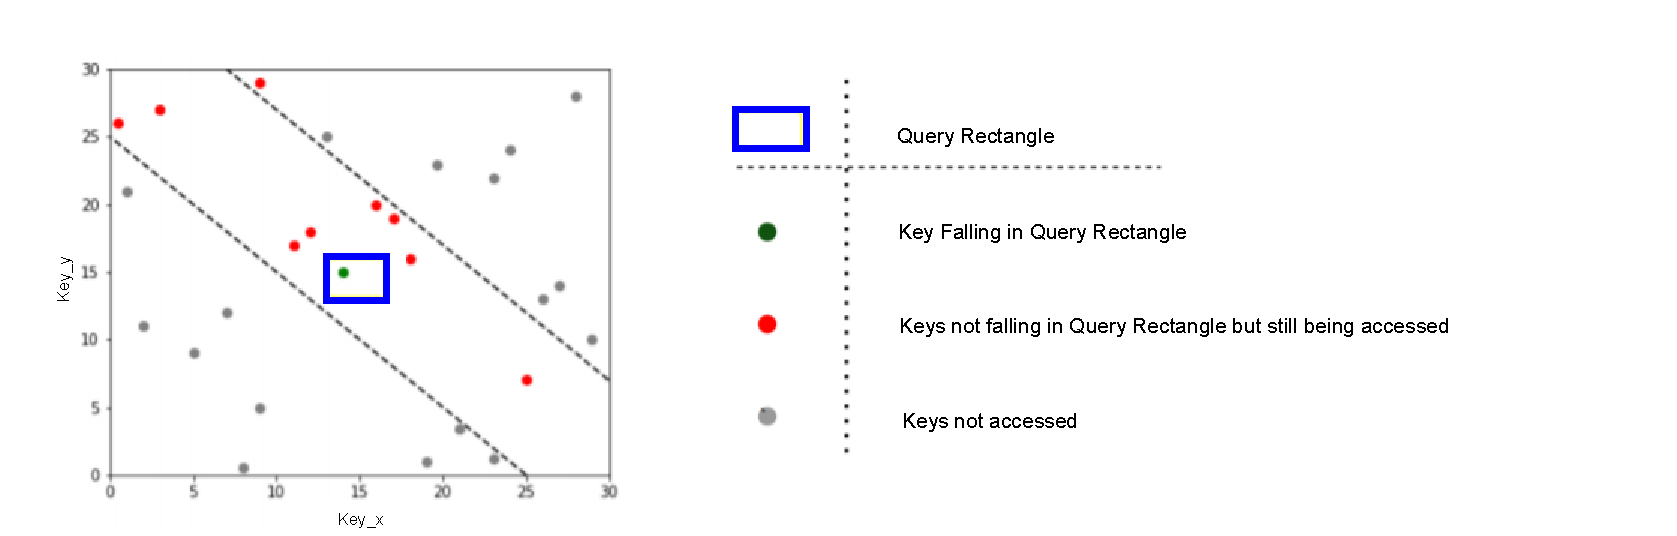
\includegraphics[width=1.3\textwidth]{graphs/Baseline_limitation.pdf}
    \caption{Baseline Method Limitation }
    \label{fig:BaseLine_Method_Limitation}
\end{figure*}
}


\subsubsection {LISA Baseline model search optimization for smaller values of N}
%In lisa baseline model, we need to linearly search for the query key in a cell. 
In case of high dimensional key values, key with in a cell can not be searched with mapped value, as a large number of keys can have the same mapped value. However for the 2 dimensional scenario, we can get considerable savings in search cost by replacing sequential scan based on keys values to binary search based on mapped value. As in the original method, search process  will consist of two parts.
\begin{enumerate}
	\item Find the cell which contains the query key based on mapped value using binary search. 
	\item With in the cell, replace sequential search based on query key value with the  binary search based on query key mapped value. Once mapped value is found, do a lookup in the neighbourhood of the found key based on query key 2 dimensional value. 
\end{enumerate}
As shown in Fig. \ref{fig:LISA_Baseline_Optimization}, we get significant savings in the query time with this approach for smaller values of N. As the value of $N$ increases, number of Keys per cell decreases, and savings in avoiding sequential search gets normalized. 


\begin{figure}
 \centering
     \begin{subfigure}[b]{0.45\textwidth}
         \centering
         \begin{tikzpicture}[font=\small]
	\pgfplotsset{compat=1.10, width=\textwidth, height=\textwidth,every axis
	legend/.append style={
		at={(1,1)},
		anchor=north east}}
	\begin{axis}[
		xmode=log,
		xlabel=$N$,
		ylabel=Average Query Time (ms),
		xtick={10,100,1000,10000},
		legend style={nodes={scale=0.55, transform shape}}
	]
	\addplot[smooth, mark=x, blue]
	coordinates{
		(10, 46.7173)
		(100, 4.8086)
		(1000, 0.7271)
		(10000,0.3301)
		%(100000,0.2381)
	};
	\addplot[smooth,mark=o,red]
  	coordinates{
        (10, 0.2855)
		(100,0.2823)
		(1000, 0.2806)
		(10000,0.2794)
		%(100000,0.2322)
	};
  
    %\legend{LISA Baseline, LISA Baseline Optimized}
	\end{axis}
\end{tikzpicture}
         \caption{Training Size 100K}
         \label{fig:2d_exp4_3_1}
     \end{subfigure}
     \begin{subfigure}[b]{0.45\textwidth}
         \centering
         \begin{tikzpicture}[font=\small]
	\pgfplotsset{compat=1.10, width=\textwidth, height=\textwidth,every axis
	legend/.append style={
		at={(1,1)},
		anchor=north east}}
	\begin{axis}[
		xmode=log,
		xlabel=$N$,
		ylabel=Average Query Time (ms),
		xtick={10,100,1000,10000},
		legend style={nodes={scale=0.75, transform shape}},
		scaled y ticks = base 10:-2,
	]
	\addplot[smooth, mark=x, blue]
	coordinates{
		(10, 347.5613)
		(100, 40.1451)
		(1000, 4.4732)
		(10000,0.6697)
		%(100000,0.2944)
	};
	\addplot[smooth,mark=o,red]
  	coordinates{
        (10, 0.2905)
		(100,0.2858)
		(1000, 0.2844)
		(10000,0.2831)
		%(100000,0.2322)
	};
  
    \legend{LISA Baseline, LISA Baseline Optimized}
	\end{axis}
\end{tikzpicture}
         \caption{Training Size 1M}
         \label{fig:2d_exp4_3_2}
     \end{subfigure}
     \caption{Point query results comparison between LISA Baseline and Optimized Model for different training sizes.}
     \label{fig:LISA_Baseline_Optimization}
\end{figure}



\chapter{Evaluation}

$K$-Nearest Neighbours ($K$NN), as the name suggests, is the process of finding $K$ nearest neighbours to a given query point. In this project, $K$NN query is only performed on $2$-dimensional data. We use $\ell_2$ norm as the distance metric. A $K$NN query will be formalised as $\mathcal{K}(\boldsymbol{X})$ where $\boldsymbol{X}\in\mathbb{R}^2$.

\subsubsection{$K$NN query with $K$D-Tree}
As a baseline, we first perform $K$NN query with $K$D-tree.\\
The main advantage of $K$D-Tree is that we can exploit the tree structure and prune points we don't think will have distance smaller than the ones we have already calculated. This improves the time complexity as compared to finding the distance of point with every other point in space to get the closest neighbours. 


\begin{algorithm}[H]
    \SetAlgoLined
    \SetKwInOut{Input}{Input}
    \SetKwInOut{Output}{Output}
    \Input{$K$; \texttt{Number of nearest neighbour, List of TestPoints; $\mathcal{P}(\boldsymbol{x}, \boldsymbol{y}); [x \in \mathbb{R};y \in \mathbb{R}]$}}
    \Output{\texttt{List of $K$ nearest points(ResultList)}}
    \For{$i\gets0$ \KwTo $len(TestPoints)$}
    {
        \texttt{Start at root}\\
        \texttt{Traverse subtree where $\mathcal{P}(\boldsymbol{x}, \boldsymbol{y})_i$ can be added.}\\
        \texttt{Find the leaf; Calculate the distance and store it as $\mathcal{D}$}\\
        \eIf{$len(ResultList) < K$}
            {
                \eIf {\texttt{Perpendicular distance of Parent with $\mathcal{P}(\boldsymbol{x}, \boldsymbol{y}) <= \mathcal{D}$}}
                    {
                        \texttt{Go on the other side of subtree} 
                    }
                        {
                            \texttt{Go up another $level$}
                        }
            }
            {
                \texttt{return ResultList}
            }
        
    }
    \caption{$K$NN Query Algorithm for $K$D-Tree}
    \label{$K$NN_Query_Algorithm_$K$D-Tree}
\end{algorithm}

In algorithm \ref{$K$NN_Query_Algorithm_$K$D-Tree},
\begin{enumerate}
    \item Start with the root to traverse tree until we reach the leaf. We find the subtree where the new $\mathcal{P}(\boldsymbol{x}, \boldsymbol{y})$ could be added and finally reach the leaf of this subtree. 

    \item Calculate the square of the euclidean distance of this point from the $\mathcal{P}(\boldsymbol{x}, \boldsymbol{y})$. We add it to the list and push and pop values from the list depending on the distances we calculate while traversing the tree upwards from here.
    
    \item From the leaf we could either go up another level or go the other side of the subtree to get a point that could have a distance smaller than the last best calculated distance in the list. 
    
    \item Once we make a decision in the above step, we can recursively traverse the tree upwards until we reach the root. 
\end{enumerate}


\begin{mscexample}


    \begin{minipage}[t]{\linewidth}
        \centering
        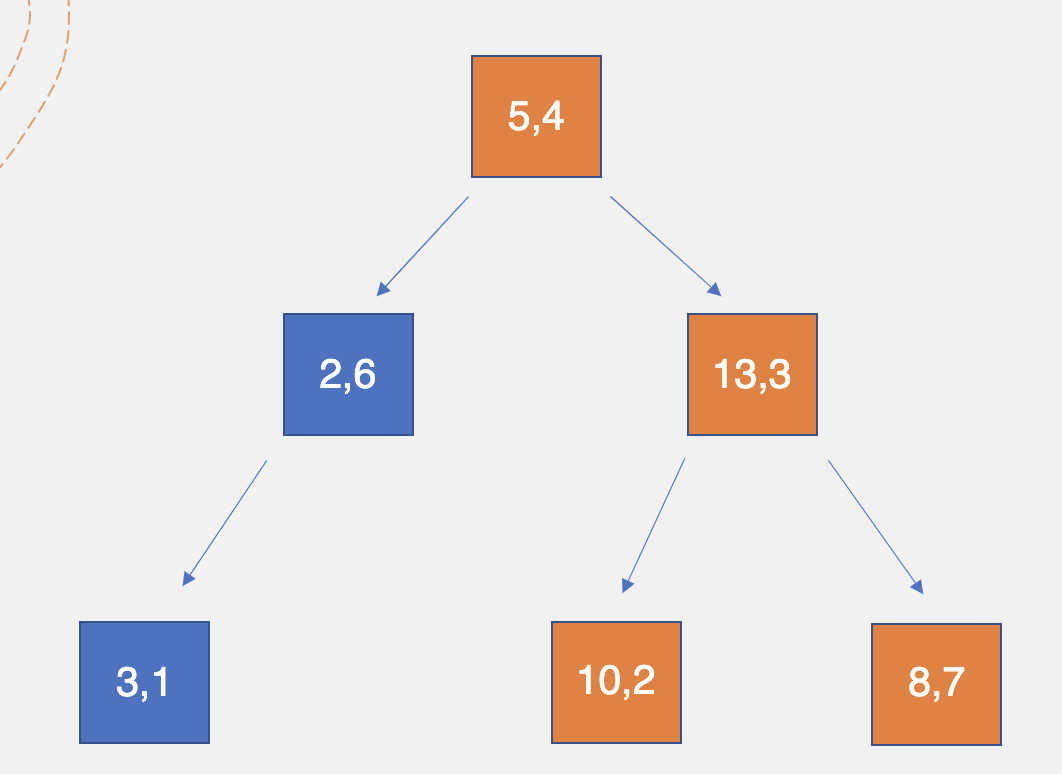
\includegraphics[width=6cm]{graphs/KD-Tree_KNN_Tree.png}
        % \caption{$K$D-Tree for KNN Query}
        \label{fig:$K$D-Tree_for_KNN Query}
        \hfill
        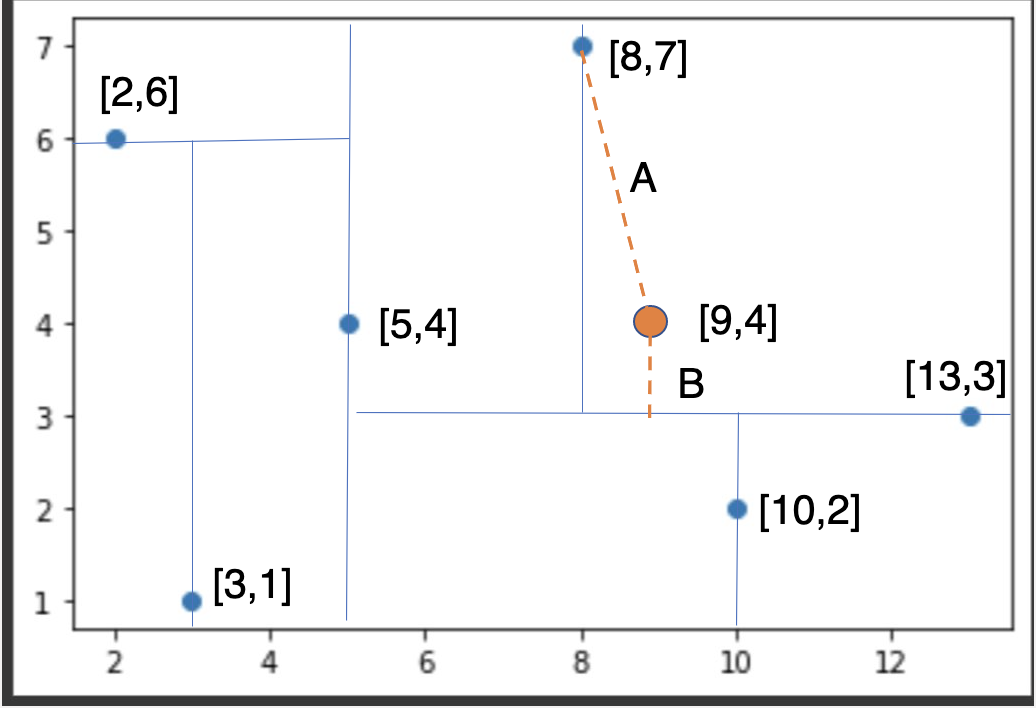
\includegraphics[width=6cm]{graphs/KD-Tree_KNN_plot.png}
        % \caption{$K$D-Tree KNN Plot on 2-dimentional plane}
        \label{fig:KD_Tree_KNN_Plot}
    \end{minipage}
	For example, we have Point list as $$((5,4),(2,6),(13,3),(8,7),(3,1),(10,2))]$$ 
	
	\textbf{Test point; $\mathcal{P}(\boldsymbol{x}, \boldsymbol{y})$} = $(9,4)$\\
	
% 	we will have a tree structure as shown in \ref{fig:$K$D-Tree_for_KNN Query} and it's plot on $2$-dimensional plane is shown in \ref{fig:KD_Tree_KNN_Plot}. *****\ref{fig:KD_Tree_KNN_Plot} \\
% 	In the fig above, we can see that although point $(8,7)$ is the leaf we will reach when we traverse the tree to search where test point $(9,4)$ can be added, it is not in fact the nearest point to the test point. \\
	
	Below are the steps followed to get the $4$ nearest neighbours:
	\begin{enumerate}
    	\item Traverse to $(8,7)$ by searching for a location where $\mathcal{P}(\boldsymbol{x}, \boldsymbol{y})$ could be added.
    	
    	\item Add $(8,7)$ to result list.
    	
    	\item Calculate the distance of $(8,7)$ and $\mathcal{P}(\boldsymbol{x}, \boldsymbol{y})$. Save the distance as $\mathcal{D}$
    	
    	\item Make a decision whether to traverse to the other side of the subtree to point $(10,2)$ by checking the perpendicular distance of $(13,3)$ with $\mathcal{P}(\boldsymbol{x}, \boldsymbol{y})$ and compare this with $\mathcal{D}$.(We do this to verify if there is even a possibility to find a point smaller than the last best distance on the other side of the subtree.) 
    	
    	\item Since the perpendicular distance is smaller than the best calculated $\mathcal{D}$ ($A > B$), we will check the distance of $\mathcal{P}(\boldsymbol{x}, \boldsymbol{y})$ and $(10,2)$. This distance in our case is indeed smaller than the best calculated distance of $\mathcal{P}(\boldsymbol{x}, \boldsymbol{y})$ with $(8,7)$ so far.
    	
    	\item Add $(10,2)$ to result list.
    	
    	\item Similarly, we traverse until we have $4$ nearest neighbour to $\mathcal{P}(\boldsymbol{x}, \boldsymbol{y})$ in the list.
	\end{enumerate}
\end{mscexample}



\subsubsection{$K$NN Query with LISA}
%TODO: What does this paragraph mean?
%We do not know the analytical representation of shards, as we use machine learning model $ \mathcal{SP}$ to generate shards. Thus, 
It is difficult to apply traditional $K$NN query pruning strategies applicable for $K$D-Trees, to LISA model as it doesn't maintain a tree like structure with all nodes and
entries based on MBRs (minimum bounding rectangle) and parent-children relationships. Shard boundaries are learned per mapped interval and no data structure is maintained to refer to shards in adjacent mapped intervals. The key idea in the $K$NN query is to convert it into a range query by estimating an appropriate query range. LISA paper suggests a learning model to learn an appropriate distance bound from underlying training data for every query point and specific value of K. However, we used empirically estimates to learn this distance bound for different values of $K$. This distance bound is used to convert the $K$NN query to range query.The query range is augmented if less than K neighbors are found in a range query. 

Consider a query point $q_{knn}=(x_{0},x_{1})$, let $x^{'} \in V$ be the $K$th nearest key to $x$ in database at a distance value $\delta = \| x^{'}-q_{knn}\|_{2} $. Lets define $ \mathcal{Q}(q_{knn},\delta) \triangleq [x_{0}-\delta, x_{0}+\delta) \times[x_{1}-\delta, x_{1}+\delta)$ and $\mathcal{B}(q_{knn}, \delta)  \triangleq \{p \in V \mid \| q_{knn}-p\|_{2} \leq \delta \} $. We can create a query rectangle $qr =  \mathcal{Q}(q_{knn}, \delta + \epsilon)$ where $\epsilon \rightarrow 0$. As shown in Fig. \ref{fig:KNN_Query_Lisa}, K nearest keys to $q_{knn}$ are all in $\mathcal{B}(q_{knn}, \delta)$ and thus in $\mathcal{Q}$. $K$NN query can be solved using the range query if we can estimate an appropriate distance bound $\delta$ for every query point.

\begin{figure*}[t]
    \centering
    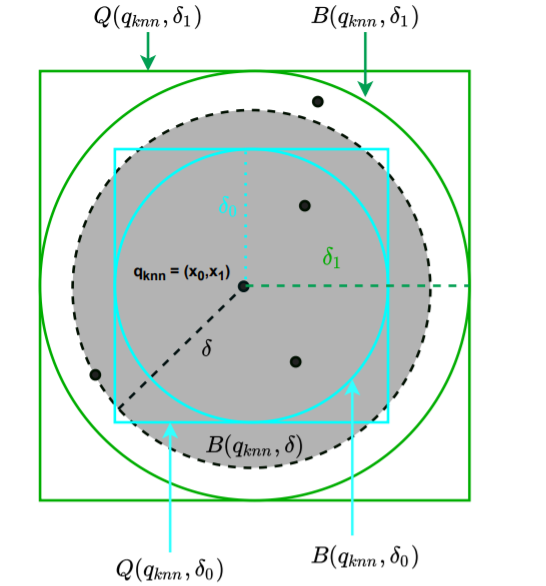
\includegraphics[width=0.7\textwidth]{graphs/KNN_Query_Lisa.png}
    \caption{KNN Query Implementation in Lisa(K=3)\\
    1)$q_{knn}$ represents the query point, $ \mathcal{Q}(x,\delta) \triangleq [x_{0}-\delta, x_{0}+\delta) \times[x_{1}-\delta, x_{1}+\delta)$, represents query rectangle and $ \mathcal{B}(x, \delta)$ represents the key space at distance $\delta$ containing K nearest keys.\\
    2)KNN query can be solved by range query if we can estimate an appropriate distance bound $\delta$ for every query point\\
    }
    \label{fig:KNN_Query_Lisa}
\end{figure*}
In our experiments, we find the $\delta$ empirically. We try with different values of $\delta$ and choose the one for which we get the best results. 

\section{One Dimensional Data and Indexes}

For one dimensional data, the evaluation covers the following tasks:

\begin{itemize}
	\item Find a structure for recursive model index empirically.
	\item Compares the performance between baseline model, recursive model and traditional B-Tree.
\end{itemize}

\subsection{Dataset}

For one dimensional case, we manually generate two columns of the data:

\begin{itemize}
	\item The first column contains the keys $X$, which is randomly sampled from a given distribution.
	\item Then we assign the keys into different pages according to a preset parameter $N_{page}$ for page size. Specifically, the first $N_{page}$ keys will be assigned into the first page, the second $N_{page}$ keys will be assigned into the second page and so on so forth. After the assignments, we set the second column $Y$ to be the page index of the corresponding $x$.
\end{itemize}

\textbf{Small Lognormal Distributed Data} We first generate $10,000$ data points where $X$ is from a lognormal distribution $\text{Lognormal}(0, 4)$. 

\begin{table}
	\centering
	\begin{tabular}{||c | c | c | c | c | c||}
		\hline
		Name& root model & 2nd model & No. of 2nd models & 3rd model & No. of 3rd models \\ [0.5ex] 
		\hline
		\hline
		Setting 1  & FCN& FCN& 200 & FCN& 2000\\
		\hline
		Setting 2  & FCN& FCN& 200 & FCN& 4000\\
		\hline
		Setting 3  & FCN& FCN& 200 & FCN& 6000\\
		\hline
		Setting 4  & FCN& FCN& 400 & FCN& 2000\\ 
		\hline
		Setting 5  & FCN& FCN& 400 & FCN& 4000\\
		\hline
		Setting 6  & FCN& FCN& 400 & FCN& 6000\\
		\hline 
		Setting 7  & FCN& FCN& 600 & FCN& 2000\\
		\hline 
		Setting 8  & FCN& FCN& 600 & FCN& 4000\\
		\hline 
		Setting 9  & FCN& FCN& 600 & FCN& 6000\\
		\hline
		Setting 10 & LR & LR& 200 & LR& 2000\\
		\hline
		Setting 11 & LR & LR& 200 & LR& 4000\\
		\hline
		Setting 12 & LR & LR& 200 & LR& 6000\\
		\hline
		Setting 13 & LR & LR& 400 & LR& 2000\\ 
		\hline
		Setting 14 & LR & LR& 400 & LR& 4000\\ 
		\hline
		Setting 15 & LR & LR& 600 & LR& 2000\\ 
		\hline
		Setting 16 & LR & LR& 600 & LR& 4000\\ 
		\hline
		Setting 17 & LR & LR& 600 & LR& 6000\\ 
		\hline
		Setting 18 & LR & LR& 400 & LR& 6000\\ 
		\hline
		Setting 19 & LR & FCN& 200 & FCN& 4000\\
		\hline
		Setting 20 & FCN& FCN& 200 & LR& 4000\\
		\hline 
		Setting 21 & FCN& LR& 200 & LR& 4000\\
		\hline 
		Setting 22 & LR & FCN& 200 & LR& 4000\\
		\hline 
		Setting 23 & FCN& LR& 200 & LR& 4000\\
		\hline
		Setting 24 & FCN& LR& 200 & LR& 4000\\
		\hline
		\hline
	\end{tabular}
	\label{small_lognormal_settings}
	\caption{Structures of recursive models for small lognormal data}
\end{table}

\begin{center}
	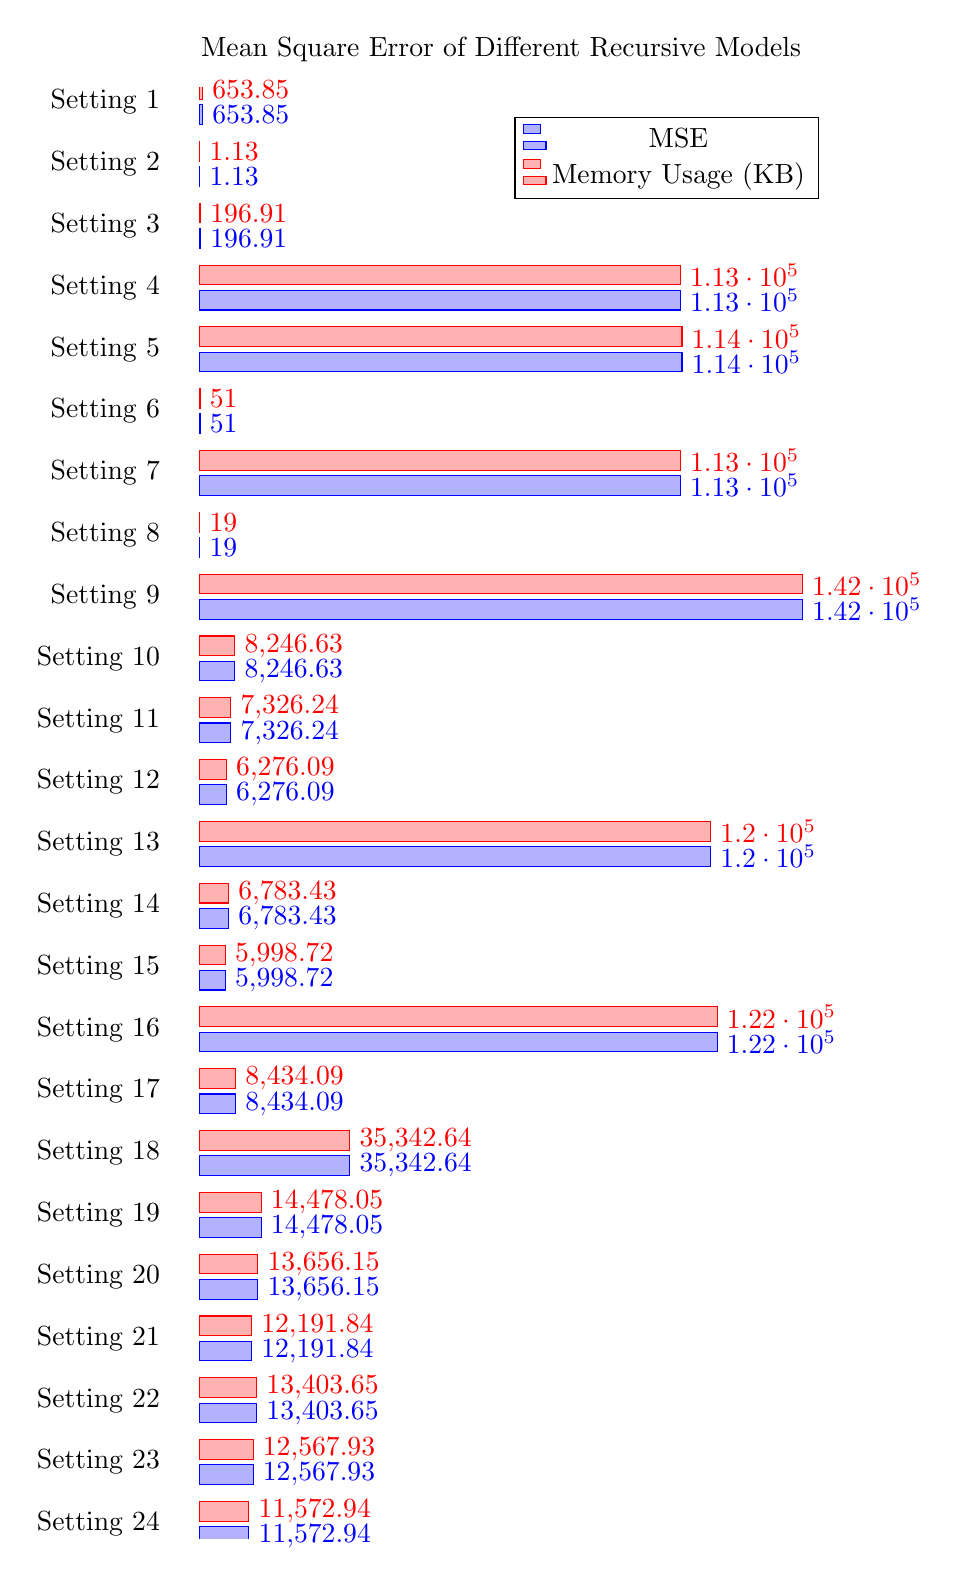
\begin{tikzpicture}
		\begin{axis}[title  = Mean Square Error of Different Recursive Models,
				xbar,
				y axis line style = { opacity = 0 },
				axis x line= none,
				ytick             = data,
				tickwidth = 0pt,
				enlarge y limits  = 0.01,
				enlarge x limits  = 0.05,
				bar width=2.5mm,
				height=20cm,
				width=10cm,
				symbolic y coords = {Setting 24, Setting 23, Setting 22, Setting 21, Setting 20, Setting 19, Setting 18, Setting 17, Setting 16, Setting 15, Setting 14, Setting 13, Setting 12, Setting 11, Setting 10, Setting 9, Setting 8, Setting 7, Setting 6, Setting 5, Setting 4, Setting 3, Setting 2, Setting 1},
				nodes near coords,
			]
			\addplot coordinates { 
			    (653.8536667,Setting 1)
				(1.134166667,Setting 2)
				(196.9116667,Setting 3)
				(113246.196,Setting 4) 
				(113652.3212,Setting 5)
				(51.00183333,Setting 6)
				(113246.2647,Setting 7)
				(18.99766667,Setting 8)
				(142041.6877,Setting 9)
				(8246.633985,Setting 10) 
				(7326.238372,Setting 11)
				(6276.09111,Setting 12)
				(120427.9247,Setting 13)
				(6783.428749,Setting 14)
				(5998.720313,Setting 15) 
				(121932.5051,Setting  16)
				(8434.091306,Setting 17)
				(35342.6365,Setting 18)
				(14478.05283,Setting 19)
				(13656.1507,Setting 20) 
				(12191.8397,Setting 21)
				(13403.64758,Setting 22)
				(12567.93278,Setting 23)
				(11572.93555,Setting 24)};
			\addplot coordinates {
				(653.8536667,Setting 1)
				(1.134166667,Setting 2)
				(196.9116667,Setting 3)
				(113246.196,Setting 4) 
				(113652.3212,Setting 5)
				(51.00183333,Setting 6)
				(113246.2647,Setting 7)
				(18.99766667,Setting 8)
				(142041.6877,Setting 9)
				(8246.633985,Setting 10) 
				(7326.238372,Setting 11)
				(6276.09111,Setting 12)
				(120427.9247,Setting 13)
				(6783.428749,Setting 14)
				(5998.720313,Setting 15) 
				(121932.5051,Setting  16)
				(8434.091306,Setting 17)
				(35342.6365,Setting 18)
				(14478.05283,Setting 19)
				(13656.1507,Setting 20) 
				(12191.8397,Setting 21)
				(13403.64758,Setting 22)
				(12567.93278,Setting 23)
				(11572.93555,Setting 24)};
			\legend{MSE, Memory Usage (KB)}
		\end{axis}
	\end{tikzpicture}
\end{center}

\textbf{Various Distributions and Sizes} After the search process for a recursive model, we then conduct experiments on several different distributions and sizes datasets. During this process, we use the following settings:

\textbf{Large Lognormal Distributed Data} The last dataset that we used is a large dataset that contains 190 million key value pairs that are distributed under lognormal distribution.

\section{Two Dimensional Data and Indexes}

For two dimensional data, the evaluation covers the following tasks:

\begin{itemize}
 	\item Find hyper-parameters for the LISA Baseline model empirically.
	\item Find hyper-parameters for the LISA model empirically.
	\item Compares the performance between $K$D-tree, LISA Baseline and LISA models for point query.
	\item Compare the performance between $K$D-tree, LISA Baseline and LISA models for range query.
	\item Compare the performance between $K$D-tree and LISA models for KNN query. $K$NN Query has not been implemented for LISA Baseline as there is no description of $K$NN Query for Baseline model in the paper. 
\end{itemize}

\subsection{Dataset}

For two dimensional case, we manually generate three columns of the data:

\begin{itemize}
	\item The first two columns contain the  2 dimensional keys $\boldsymbol{X} \in \mathbb{R}^{2}$, which are independently sampled from Lognormal Distribution. Data set  
contains 190 million key value pairs.
	\item Then we assign the keys into different pages according to a preset parameter $N_{page}$ for page size. Specifically, the first $N_{page}$ keys will be assigned into the first page, the second $N_{page}$ keys will be assigned into the second page and so on so forth. After the assignments, we set the second column $Y$ to be the page index of the corresponding $x$.
\end{itemize}

Our final data-set consists of 190 million key value pairs that are distributed under log-normal distribution
As discussed in previous section, there are multiple challenges in using  the complete data-set for training and hyper-parameters tuning. Even on google cloud server, running experiments with the full data take considerable long times (Lisa model took 26 hours to build), we had limited cloud server budget and a large number of experiments to run. Therefore, for two dimensional indexes evaluation, we have used sampling to generate smaller training datasets.   


\subsection{Hyper-parameters Search}
After generating dataset as mentioned in previous section, we sample a smaller subset from it. We repeat our experiments for 3 different sample sizes of 10000, 100000 and 1000000 points. Test data is a copy of training data for all our experiments. For Baseline and Lisa models, final prediction is given by linear search through a range of values (identified as a Cell for Baseline and Shard for LISA model) and mean square error (MSE) is zero as test points are already learned during training. This is where Learned Index models differ from traditional machine learning models where model performance is evaluated on unseen data. 

\subsubsection {Hyper-parameter search for the LISA Baseline implementation}
Baseline model has one hyper-parameter: N (Number of cells specifying the number of equal length intervals into which mapped values are divided). The point query search consists of two parts, first is binary search to locate the cell into which the query key is located, followed by sequentially comparison of the query key value with keys in the found cell until a match is found. The time complexity of first search is $log_{2}N_{1}$, where $N_{1}$ is the number of cells. The time complexity of second search is  $ \left \lceil {N_{2} / 2}\right \rceil $, where $N_{2}$ is the number of keys per cell.  

\begin{figure}
 \centering
     \begin{subfigure}[b]{0.32\textwidth}
         \centering
         \begin{tikzpicture}[font=\small]
	\pgfplotsset{compat=1.10, width=\textwidth, height=\textwidth,every axis
	legend/.append style={
		at={(1,1)},
		anchor=north east}}
	\begin{axis}[
		xmode=log,
		xlabel=$N$,
		ylabel=Average Query Time (ms),
		xtick={10,100,1000,10000},
		legend style={nodes={scale=0.55, transform shape}}
	]
	\addplot[smooth, mark=x, blue]
	coordinates{
		(10, 4.34261)
		(100,0.71891)
		(1000, 0.32806)
		(10000,0.24157)
	};
	\addplot[smooth,mark=o,red]
  	coordinates{
    	(10, 46.7173)
		(100, 4.8086)
		(1000, 0.7271)
		(10000,0.3301)
	};
    \addplot[smooth,mark=+,black!60!green]
    coordinates{
      (10,347.561)
      (100,40.145)
      (1000,4.473)
      (10000,0.669)
    };
    \legend{10K,100K,1M}
	\end{axis}
\end{tikzpicture}
         \caption{Average Query Time (ms)}
         \label{fig:2d_exp3_1_1}
     \end{subfigure}
     \hfill
     \begin{subfigure}[b]{0.32\textwidth}
         \centering
         \begin{tikzpicture}[font=\small]
	\pgfplotsset{compat=1.10, width=\textwidth, height=\textwidth}
	\begin{axis}[
		xmode=log,
		xlabel=$N$,
		ylabel=Memory Size(KB),
		xtick={10,100,1000,10000}
	]
	\addplot[smooth, mark=x, blue]
	coordinates{
		(10, 313)
		(100, 315)
		(1000, 336)
		(10000,547)
	};
	\addplot[smooth,mark=o,red]
  	coordinates{
    	(10, 3126)
		(100, 3128)
		(1000, 3149)
		(10000,3360)
	};
    \addplot[smooth,mark=+,black!60!green]
    coordinates{
      (10,31251)
      (100,31253)
      (1000,31274)
      (10000,31485)
    };
	\end{axis}
\end{tikzpicture}
         \caption{Memory Size (KB)}
         \label{fig:2d_exp3_1_2}
     \end{subfigure}
     \hfill
     \begin{subfigure}[b]{0.32\textwidth}
         \centering
         \begin{tikzpicture}[font=\small]
	\pgfplotsset{compat=1.10, width=\textwidth, height=\textwidth}
	\begin{axis}[
		xmode=log,
		xlabel=$N$,
		ylabel=Build  Time(s),
		xtick={10,100,1000,10000},
		scaled y ticks = base 10:-2,
	]
	\addplot[smooth, mark=x, blue]
	coordinates{
		(10, 11.171)
		(100, 11.252)
		(1000, 13.542)
		(10000,26.831)
	};
	\addplot[smooth,mark=o,red]
  	coordinates{
    	(10,109.287)
    	(100,111.596)
    	(1000,111.978)
    	(10000,128.496)
	};
    \addplot[smooth,mark=+,black!60!green]
    coordinates{
      (10,1094.99)
      (100,1099.68)
      (1000,1104.63)
      (10000,1143.73)
    };
	\end{axis}
\end{tikzpicture}
         \caption{Build Time (s)}
         \label{fig:2d_exp3_1_3}
     \end{subfigure}
     \hfill
     \caption{Hyper-parameter search in LISA Baseline for training sizes $10K$, $100K$ and $1M$.}
     \label{fig:LISA_Baseline_Hyperparameter_Search}
\end{figure}


\begin{mscconclusion}
	Following conclusions can be drawn from experimental results shown in table \ref{small_lognormal_lisa_baseline_10000} and Fig. \ref{fig:LISA_Baseline_Hyperparameter_Search}
\begin{enumerate}
    \item Optimum value of hyper-parameter N will be equal to number of points in the training data-set, resulting in 1 key per cell and search query time of O($log_{2}N$).
	
	\item Average Query Time:  Average Query Time decreases with increase in value of N as number of keys per cell decreases.
	\item Build time: Build time increases with increase in value of N, as metadata for additional cells needs to be calculated. 
	\item Memory Size:  Memory requirements of the model increases with increase in value of N, as metadata for additional cells needs to be stored. Increase  in memory size is not significant with increase in N as we maintain only two values per cell, mapped value of first key in the cell and mapped value of last key in the cell.
\end{enumerate}
\end{mscconclusion}

\subsubsection {Hyper-parameter search for the LISA implementation}
For LISA model, we have 3 hyper parameters:
\begin{enumerate}
	\item $G$: The size of the grid cell. Number of grid cells into which the key space is divided. In our implementation, we use a square grid cell, and total number of cells is given by $G$ $\times G$.
	\item $N$: Number of equal length intervals into which mapped value range is divided. During our experiments, we found that shard prediction algorithm gives better performance if mapped interval boundaries are aligned to grid cell boundaries. That's why this parameter is always initialised to $N$=$G$ $\times G$   
	\item $S$: Number of shards to learn per mapped interval. 
\end{enumerate}

\begin{mscconclusion}
	Following conclusions can be drawn from experiments results shown in tables \ref{small_lognormal_lisa_10000}, \ref{small_lognormal_lisa_100000} and \ref{small_lognormal_lisa_1000000}. 
\begin{enumerate}

    \item For a particular value of $G$, average query time decreases and memory size increases with increase in value of S. This is expected as increasing S, will result in lesser number of keys per shard, thereby reducing the sequential search cost of scanning the query key through the Shard. 
    
    \item Average query time decreases and memory size increases with increase in values of $G$ and $S$. 
	
	\item We found emprically that value of $S$ should be choosen such that there are at least 45 keys per shard. We see mean square errors(mse) if number of keys per shard are less than 45 for following reasons. 
	\begin{enumerate}
	    \item For point query search, we first predict a shard and then sequentially compare the query point key values with all the keys in the predicted shard until a match is found
		\item For query points near the shard boundaries, there can be a mismatch in ground truth shard-id and predicted shard-id.If the query point is not found in the predicted shard, we continue our search in adjacent left and right shards in an empirically found range.
	\end{enumerate}
	
	During test experiments, we found that if shard size is less than 45 keys, sometimes shard prediction error can be greater than 1 and point query search can fail resulting in MSE errors.  
\end{enumerate}
\end{mscconclusion}

\subsection{Comparisons Across Models}

During following experiments, for each training data size, we have used hyper-parameters optimized for that particular data set size. 

\subsubsection{Point Query Comparison}
Table \ref{Point_Query_Comparision} and  Fig. \ref{fig:Point_Query_Comparision} shows the performance evaluation for $K$D-Tree, LISA-Baseline and LISA Models for different training data sizes. For a given training set, we perform point query evaluation for every point in the data-set and take the average. 

\begin{figure}
 	 \centering
     \begin{subfigure}[b]{0.32\textwidth}
         \centering
         \begin{tikzpicture}[font=\small]
	\pgfplotsset{compat=1.10, width=\textwidth, height=\textwidth,every axis
	legend/.append style={
		at={(1,0)},
		anchor=south east}}
	\begin{axis}[
		xmode=log,
		xlabel=Training Size,
		ylabel=Average Query Time (ms),
		xtick={10000,100000,1000000,10000000},
		legend style={nodes={scale=0.35, transform shape}}
	]
	\addplot[smooth, mark=x, blue]
	coordinates{
		(10000, 4.363)
		(100000, 6.176)
		(1000000, 9.254)
		(10000000,11.254)
	};
	\addplot[smooth,mark=o,red]
  	coordinates{
    	(10000,0.198)
    	(100000,0.281)
    	(1000000,0.543)
    	(10000000,1.616)
	};
    \addplot[smooth,mark=+,black!60!green]
    coordinates{
      (10000,0.861)
      (100000,1.432)
      (1000000,1.645)
      (10000000,2.972)
    };
	\end{axis}
\end{tikzpicture}
         \caption{Average Query Time (ms)}
         \label{fig:2d_exp2_1_1}
     \end{subfigure}
     \hfill
     \begin{subfigure}[b]{0.32\textwidth}
         \centering
         \begin{tikzpicture}[font=\small]
	\pgfplotsset{compat=1.10, width=\textwidth, height=\textwidth,every axis
	legend/.append style={
		at={(1,0)},
		anchor=south east}}
	\begin{axis}[
		xmode=log,
		xlabel=Training Size,
		ylabel=Memory Size (KB),
		xtick={10000,100000,1000000,10000000},
		legend style={nodes={scale=0.4, transform shape}}
	]
	\addplot[smooth, mark=x, blue]
	coordinates{
		(10000, 2890)
		(100000, 28906)
		(1000000, 289062)
		(10000000, 2821880)
	};
	\addplot[smooth,mark=o,red]
  	coordinates{
    	(10000,547)
    	(100000,5469)
    	(1000000,54688)
    	(10000000,547792)
	};
    \addplot[smooth,mark=+,black!60!green]
    coordinates{
      (10000,337)
      (100000,3169)
      (1000000,32477)
      (10000000,328142)
    };
    %\legend{$K$D-Tree,Baseline,LISA}
	\end{axis}
	 
\end{tikzpicture}
         \caption{Memory Size (KB)}
         \label{fig:2d_exp2_1_2}
     \end{subfigure}
     \hfill
     \begin{subfigure}[b]{0.32\textwidth}
         \centering
         \begin{tikzpicture}[font=\small]
	\pgfplotsset{compat=1.10, width=\textwidth, height=\textwidth, every axis legend/.append style={
		at={(0,1)},
		anchor=north west}}
	\begin{axis}[
		xmode=log,
		%ymode=log,
		xlabel=Training Size,
		ylabel=Build Time (s),
		xtick={10000,100000,1000000,10000000},
		legend style={nodes={scale=0.4, transform shape}}
	]
	\addplot[smooth, mark=x, blue]
	coordinates{
		(10000, 0.023)
		(100000, 0.340)
		(1000000, 4.124)
		(10000000, 77.991)
	};
	\addplot[smooth,mark=o,red]
  	coordinates{
    	(10000,0.026)
    	(100000,0.324)
    	(1000000,2.718)
    	(10000000, 13.136)
	};
    \addplot[smooth,mark=+,black!60!green]
    coordinates{
      (10000,1.127)
      (100000,22.491)
      (1000000,445.324)
      (10000000,  4730.621)
    };
	\legend{$K$D-Tree,Baseline,LISA}
	\end{axis}
\end{tikzpicture}
         \caption{Build Time (s)}
         \label{fig:2d_exp2_1_3}
     \end{subfigure}
     \hfill
     \caption{Point Query experimental results for $K$D-Tree, Baseline and LISA models.}
     \label{fig:Point_Query_Comparision}
\end{figure}

\begin{mscconclusion}
The following conclusions can be concluded:

	\begin{enumerate}
    \item LISA outperforms $K$D-tree in terms of average query time. Search complexity of $K$D-Tree and LISA baseline( configured to keep 1 key per cell) is $O(N)$, and O($log_{2}N$) respectively where N is the number of points in the training data-set. On the other hand point query search cost in LISA is a combination of 4 costs.
    \begin{enumerate}
    \item Search cost to find the grid cell to which point query belongs. This cost increase linearly with increase in number of grid cells. 
    %Once the grid cell is found, calculate the mapped value as specified in the section.
    \item Search cost to find the mapped interval to which point query belongs. Search complexity of this cost is O($log_{2}U$), where U is the number of intervals into which sorted mapped array is divided. 
    
    \item Find the shard-id to which point query belongs. This cost is constant as shard prediction function weights are already learned during the build process. 
    
    \item Once the shard Id is found, search sequentially in the shard interval by comparing query point key value with all the keys in the shard until a match is found. This cost is relatively constant with respect to increase in training data-size as we try to initialize our hyper-parameters in such a way that number of keys per shard remain close to 50. 
\end{enumerate}
    
    \item LISA outperforms $K$D-tree in terms of memory size requirements. The storage consumption of LISA is considerably smaller than $K$D-Tree that has to construct a tree with all nodes and entries based on MBRs (minimum bounding rectangle)  and parent-children relationships. In contrast, LISA only keeps the parameters of $M$ and $SP$. Specifically,$M$’s parameters contain several numbers and a small list only, and $SP$ is composed of a series of piecewise linear functions whose parameters are a number of coefficients.
    
    \item LISA's build time is significantly higher than $K$D-Tree and LISA Baseline. The higher build time is caused by Shard Training Algorithm.  
\end{enumerate}

\end{mscconclusion}

\subsubsection {Range Query Experiments}
Table \ref{Range_Query_Experimental_Results} shows evaluation results for LISA,Baseline and $K$D-tree models for range sizes of 10, 100, 1000 for different training sizes. For a given range query size, we perform 20 trials and take the average. For each trial, we sample a random point from the test set and find the range from sampled point to the range query size. Average query time for each range is further divided by the range size to compare the query time across various ranges. As shown in the Fig. \ref{fig:Range_Query_Comparision}, LISA outperforms $K$D-tree for range query size of 10000 for all training sizes, however its range query time for smaller range sizes is significantly higher than $K$D-Tree.

\begin{figure}
 \centering
     \begin{subfigure}[b]{0.45\textwidth}
         \centering
         \begin{tikzpicture}[font=\small]
	\pgfplotsset{compat=1.10, width=\textwidth, height=\textwidth}
	\begin{axis}[
		xmode=log,
        %ymode=log,
		xlabel=Range Query Size,
		ylabel=Average Query Time (ms),
		xtick={10,100,1000, 10000},
	]
	\addplot[smooth, mark=x, blue]
	coordinates{
		(10, 0.2238)
		(100, 0.0922)
		(1000, 0.0696)
		(10000, 0.0744)
	};
	\addplot[smooth,mark=o,red]
	coordinates{
		(10, 0.2661)
		(100, 0.0617)
		(1000, 0.0437)
		(10000, 0.0412)
	};
    \addplot[smooth,mark=+,black!60!green]
	coordinates{
		(10, 3.5181)
		(100, 0.6263)
		(1000, 0.0939)
		(10000, 0.0186)
	};
	\end{axis}
\end{tikzpicture}
         \caption{Range Query Size}
         \label{fig:2d_exp2_2_1}
     \end{subfigure}
     \hfill
     \begin{subfigure}[b]{0.45\textwidth}
         \centering
         \begin{tikzpicture}[font=\small]
	\pgfplotsset{compat=1.10, width=\textwidth, height=\textwidth, every axis legend/.append style={
		at={(1,0)},
		anchor=south east}}
	\begin{axis}[
		xmode=log,
        %ymode=log,
		xlabel=Training Size,
		ylabel=Average Query Time (ms),
		xtick={10000, 100000,1000000},
		legend style={nodes={scale=1, transform shape}}
	]
	\addplot[smooth, mark=x, blue]
	coordinates{
		(10000, 0.0648)
		(100000, 0.0718)
		(1000000, 0.0735)
	};
	\addplot[smooth,mark=o,red]
	coordinates{
		(10000, 0.0382)
		(100000, 0.0392)
		(1000000, 0.0412)
	};
    \addplot[smooth,mark=+,black!60!green]
	coordinates{
		(10000, 0.0061)
		(100000, 0.0129)
		(1000000, 0.0186)
	};
	\legend{$K$D-Tree,Baseline,LISA}
	\end{axis}
\end{tikzpicture}
         \caption{Training Size}
         \label{fig:2d_exp2_2_2}
     \end{subfigure}
     \hfill
     \caption{Range Query experimental results for $K$D-Tree, Baseline and LISA models}
        \label{fig:Range_Query_Comparision}
\end{figure}

\begin{figure}
 \centering
     \begin{subfigure}[h]{0.45\textwidth}
         \centering
         \begin{tikzpicture}[font=\small]
	\pgfplotsset{compat=1.10, width=\textwidth, height=\textwidth}
	\begin{axis}[
		xlabel=$K$,
		ylabel=Average Query Time (ms),
		xtick={3, 5, 7, 10},
	]
	\addplot[smooth, mark=x, blue]
	coordinates{
		(3, 2.7865)
		(5, 1.7072)
		(7, 1.3255)
		(10, 0.9172)
	};
	\addplot[smooth,mark=+,black!60!green]
	coordinates{
		(3, 1.2181)
		(5, 0.9414)
		(7, 0.7681)
		(10, 0.4779)
	};
	\end{axis}
\end{tikzpicture}
         \caption{Number of Nearest Neighbours ($K$)}
         \label{fig:2d_exp2_3_1}
     \end{subfigure}
     \begin{subfigure}[h]{0.45\textwidth}
         \centering
         \begin{tikzpicture}[font=\small]
	\pgfplotsset{compat=1.10, width=\textwidth, height=\textwidth, every axis legend/.append style={
		at={(1,0)},
		anchor=south east}}
	\begin{axis}[
		xmode=log,
		xlabel=Training Size,
		ylabel=Average Query Time (ms),
		xtick={10000, 100000,1000000},
		legend style={nodes={scale=1, transform shape}}
	]
	\addplot[smooth, mark=x, blue]
	coordinates{
		(10000, 0.4368)
		(100000, 0.6618)
		(1000000, 0.9172)
	};
	\addplot[smooth,mark=+,black!60!green]
	coordinates{
		(10000, 0.0549)
		(100000, 0.2161)
		(1000000, 0.4779)
	};
	\legend{$K$D-Tree,LISA}
	\end{axis}
\end{tikzpicture}
         \caption{Training Size (Fix $K=10$)}
         \label{fig:2d_exp2_3_2}
     \end{subfigure}
     \caption{$K$NN Query experimental results for $K$D-Tree and LISA models}
     %Lisa outperforms $K$D-Tree for all training data sizes. }
        \label{fig:KNN_Query_Comparision}
\end{figure}

\subsubsection {$K$NN Query Experiments}
Table \ref{KNN_Query_Experimental_Results} shows evaluation results for LISA and $K$D-tree models for $K$NN Queries for various value of K and training sizes. For a given $K$ value, we perform 20 trials and take the average of query time. For each trial, we sample a random point from the test set and find K neighbours around that point. Average query Time is further divided by $K$ to compare the Query time across various values of $K$.As shown in the Fig. \ref{fig:KNN_Query_Comparision}, LISA outperforms $K$D-tree for different training sizes and K values.




\chapter{Insights and Findings}

\section{General Discussions}

$K$-Nearest Neighbours ($K$NN), as the name suggests, is the process of finding $K$ nearest neighbours to a given query point. In this project, $K$NN query is only performed on $2$-dimensional data. We use $\ell_2$ norm as the distance metric. A $K$NN query will be formalised as $\mathcal{K}(\boldsymbol{X})$ where $\boldsymbol{X}\in\mathbb{R}^2$.

\subsubsection{$K$NN query with $K$D-Tree}
As a baseline, we first perform $K$NN query with $K$D-tree.\\
The main advantage of $K$D-Tree is that we can exploit the tree structure and prune points we don't think will have distance smaller than the ones we have already calculated. This improves the time complexity as compared to finding the distance of point with every other point in space to get the closest neighbours. 


\begin{algorithm}[H]
    \SetAlgoLined
    \SetKwInOut{Input}{Input}
    \SetKwInOut{Output}{Output}
    \Input{$K$; \texttt{Number of nearest neighbour, List of TestPoints; $\mathcal{P}(\boldsymbol{x}, \boldsymbol{y}); [x \in \mathbb{R};y \in \mathbb{R}]$}}
    \Output{\texttt{List of $K$ nearest points(ResultList)}}
    \For{$i\gets0$ \KwTo $len(TestPoints)$}
    {
        \texttt{Start at root}\\
        \texttt{Traverse subtree where $\mathcal{P}(\boldsymbol{x}, \boldsymbol{y})_i$ can be added.}\\
        \texttt{Find the leaf; Calculate the distance and store it as $\mathcal{D}$}\\
        \eIf{$len(ResultList) < K$}
            {
                \eIf {\texttt{Perpendicular distance of Parent with $\mathcal{P}(\boldsymbol{x}, \boldsymbol{y}) <= \mathcal{D}$}}
                    {
                        \texttt{Go on the other side of subtree} 
                    }
                        {
                            \texttt{Go up another $level$}
                        }
            }
            {
                \texttt{return ResultList}
            }
        
    }
    \caption{$K$NN Query Algorithm for $K$D-Tree}
    \label{$K$NN_Query_Algorithm_$K$D-Tree}
\end{algorithm}

In algorithm \ref{$K$NN_Query_Algorithm_$K$D-Tree},
\begin{enumerate}
    \item Start with the root to traverse tree until we reach the leaf. We find the subtree where the new $\mathcal{P}(\boldsymbol{x}, \boldsymbol{y})$ could be added and finally reach the leaf of this subtree. 

    \item Calculate the square of the euclidean distance of this point from the $\mathcal{P}(\boldsymbol{x}, \boldsymbol{y})$. We add it to the list and push and pop values from the list depending on the distances we calculate while traversing the tree upwards from here.
    
    \item From the leaf we could either go up another level or go the other side of the subtree to get a point that could have a distance smaller than the last best calculated distance in the list. 
    
    \item Once we make a decision in the above step, we can recursively traverse the tree upwards until we reach the root. 
\end{enumerate}


\begin{mscexample}


    \begin{minipage}[t]{\linewidth}
        \centering
        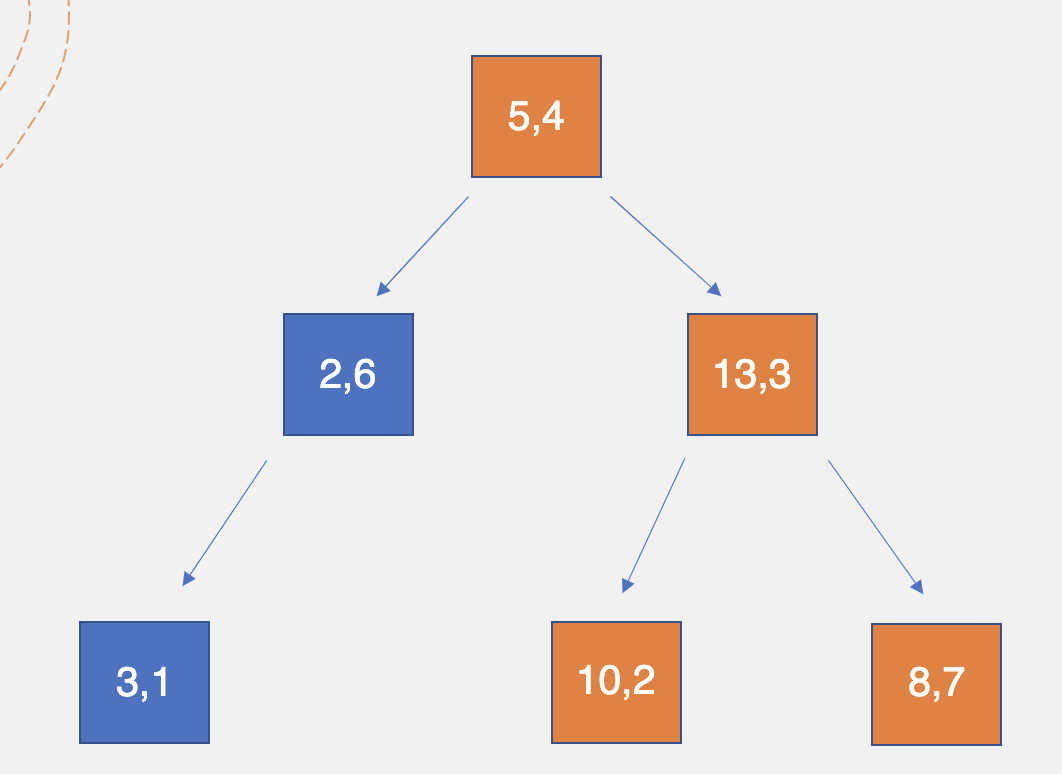
\includegraphics[width=6cm]{graphs/KD-Tree_KNN_Tree.png}
        % \caption{$K$D-Tree for KNN Query}
        \label{fig:$K$D-Tree_for_KNN Query}
        \hfill
        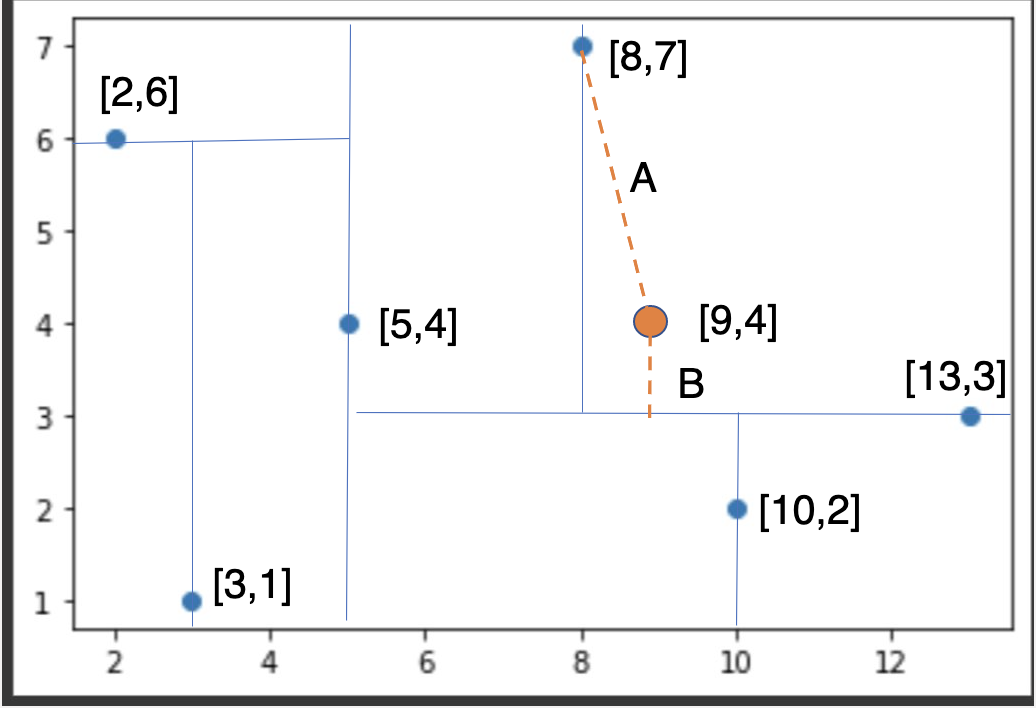
\includegraphics[width=6cm]{graphs/KD-Tree_KNN_plot.png}
        % \caption{$K$D-Tree KNN Plot on 2-dimentional plane}
        \label{fig:KD_Tree_KNN_Plot}
    \end{minipage}
	For example, we have Point list as $$((5,4),(2,6),(13,3),(8,7),(3,1),(10,2))]$$ 
	
	\textbf{Test point; $\mathcal{P}(\boldsymbol{x}, \boldsymbol{y})$} = $(9,4)$\\
	
% 	we will have a tree structure as shown in \ref{fig:$K$D-Tree_for_KNN Query} and it's plot on $2$-dimensional plane is shown in \ref{fig:KD_Tree_KNN_Plot}. *****\ref{fig:KD_Tree_KNN_Plot} \\
% 	In the fig above, we can see that although point $(8,7)$ is the leaf we will reach when we traverse the tree to search where test point $(9,4)$ can be added, it is not in fact the nearest point to the test point. \\
	
	Below are the steps followed to get the $4$ nearest neighbours:
	\begin{enumerate}
    	\item Traverse to $(8,7)$ by searching for a location where $\mathcal{P}(\boldsymbol{x}, \boldsymbol{y})$ could be added.
    	
    	\item Add $(8,7)$ to result list.
    	
    	\item Calculate the distance of $(8,7)$ and $\mathcal{P}(\boldsymbol{x}, \boldsymbol{y})$. Save the distance as $\mathcal{D}$
    	
    	\item Make a decision whether to traverse to the other side of the subtree to point $(10,2)$ by checking the perpendicular distance of $(13,3)$ with $\mathcal{P}(\boldsymbol{x}, \boldsymbol{y})$ and compare this with $\mathcal{D}$.(We do this to verify if there is even a possibility to find a point smaller than the last best distance on the other side of the subtree.) 
    	
    	\item Since the perpendicular distance is smaller than the best calculated $\mathcal{D}$ ($A > B$), we will check the distance of $\mathcal{P}(\boldsymbol{x}, \boldsymbol{y})$ and $(10,2)$. This distance in our case is indeed smaller than the best calculated distance of $\mathcal{P}(\boldsymbol{x}, \boldsymbol{y})$ with $(8,7)$ so far.
    	
    	\item Add $(10,2)$ to result list.
    	
    	\item Similarly, we traverse until we have $4$ nearest neighbour to $\mathcal{P}(\boldsymbol{x}, \boldsymbol{y})$ in the list.
	\end{enumerate}
\end{mscexample}



\subsubsection{$K$NN Query with LISA}
%TODO: What does this paragraph mean?
%We do not know the analytical representation of shards, as we use machine learning model $ \mathcal{SP}$ to generate shards. Thus, 
It is difficult to apply traditional $K$NN query pruning strategies applicable for $K$D-Trees, to LISA model as it doesn't maintain a tree like structure with all nodes and
entries based on MBRs (minimum bounding rectangle) and parent-children relationships. Shard boundaries are learned per mapped interval and no data structure is maintained to refer to shards in adjacent mapped intervals. The key idea in the $K$NN query is to convert it into a range query by estimating an appropriate query range. LISA paper suggests a learning model to learn an appropriate distance bound from underlying training data for every query point and specific value of K. However, we used empirically estimates to learn this distance bound for different values of $K$. This distance bound is used to convert the $K$NN query to range query.The query range is augmented if less than K neighbors are found in a range query. 

Consider a query point $q_{knn}=(x_{0},x_{1})$, let $x^{'} \in V$ be the $K$th nearest key to $x$ in database at a distance value $\delta = \| x^{'}-q_{knn}\|_{2} $. Lets define $ \mathcal{Q}(q_{knn},\delta) \triangleq [x_{0}-\delta, x_{0}+\delta) \times[x_{1}-\delta, x_{1}+\delta)$ and $\mathcal{B}(q_{knn}, \delta)  \triangleq \{p \in V \mid \| q_{knn}-p\|_{2} \leq \delta \} $. We can create a query rectangle $qr =  \mathcal{Q}(q_{knn}, \delta + \epsilon)$ where $\epsilon \rightarrow 0$. As shown in Fig. \ref{fig:KNN_Query_Lisa}, K nearest keys to $q_{knn}$ are all in $\mathcal{B}(q_{knn}, \delta)$ and thus in $\mathcal{Q}$. $K$NN query can be solved using the range query if we can estimate an appropriate distance bound $\delta$ for every query point.

\begin{figure*}[t]
    \centering
    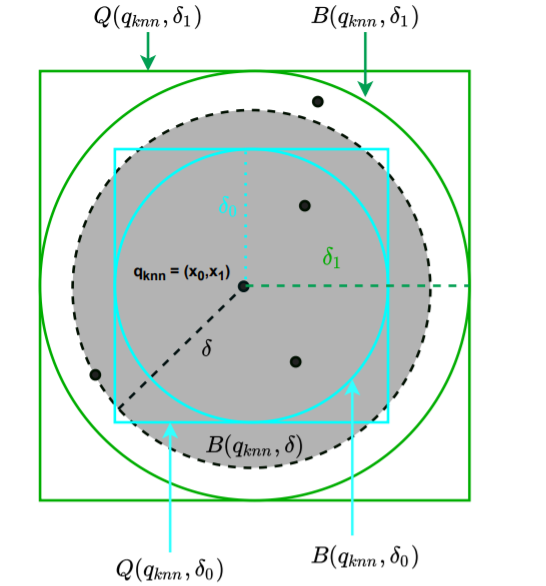
\includegraphics[width=0.7\textwidth]{graphs/KNN_Query_Lisa.png}
    \caption{KNN Query Implementation in Lisa(K=3)\\
    1)$q_{knn}$ represents the query point, $ \mathcal{Q}(x,\delta) \triangleq [x_{0}-\delta, x_{0}+\delta) \times[x_{1}-\delta, x_{1}+\delta)$, represents query rectangle and $ \mathcal{B}(x, \delta)$ represents the key space at distance $\delta$ containing K nearest keys.\\
    2)KNN query can be solved by range query if we can estimate an appropriate distance bound $\delta$ for every query point\\
    }
    \label{fig:KNN_Query_Lisa}
\end{figure*}
In our experiments, we find the $\delta$ empirically. We try with different values of $\delta$ and choose the one for which we get the best results. 

\section{One Dimensional Learned Index}

\subsection{Baseline Learned Index}

\subsubsection{Activation Functions}
\begin{itemize}
\item
  If we use identity activation function, i.e.$z^{(i)}(x)=x$, then no
  matter how many layers are there, the fully connected neural network
  falls back to a linear regression.

  \textbf{Proof:} The output of the first layer, with identity
  activation function, will be
  \(z^{(1)}(w^{(1)}x+b^{(1)})=w^{(1)}x+b^{(1)}\). Then the output will
  be the input of the next layer, and hence the output of the second
  layer will be
  \(z^{(2)}(w^{(2)}(w^{(1)}x+b^{(1)})+b^{(2)})=w^{(2)}w^{(1)}x+w^{(2)}b^{(1)}+b^{(2)}\).
  Similar induction can be obtained for multiple layers. Hence if we use
  identity activation, the trained neural network will fall back to a
  linear regression. 
\item
  With ReLU (Rectified Linear Unit) as activation function
  i.e.~\(z^{(i)}(x)=\text{max}(0,x)\), then the fully connected neural
  network falls back to a piecewise linear function.

  \textbf{Proof:} The output with ReLU activation function, will be
  \(z^{(1)}(w^{(1)}x+b^{(1)})=\text{max}(w^{(1)}x+b^{(1)}, 0)\). Then
  the output will be the input of the next layer, and hence the output
  of the second layer will be
  \(z^{(2)}(w^{(2)}(w^{(1)}x+b^{(1)})+b^{(2)})=\text{max}(w^{(2)}w^{(1)}x+w^{(2)}b^{(1)}+b^{(2)},0)\).
  Similar induction can be obtained for multiple layers. Hence if we use
  identity activation, the trained neural network will fall back to a
  piecewise linear function. The visualization below shows our lemma is
  correct.
\end{itemize}

\section{Two Dimensional Learned Index}

\comm{
\subsubsection{LISA Baseline model Limitation}

Prediction cost in baseline method consists of following two parts.

\begin{enumerate}
	\item Search cost for the cell which contains the key. This cost will be equal to $log_{2}N_{1}$, where $N_{1}$ is the number of cells into which mapped values are divided.
	
	\item Cost associated with sequentially comparing the query point key value against keys inside the cell found in previous search. On average this cost will be equal to $N_{2}\slash2$, where $N_{2}$ is the number of keys in a cell.   
	
If cell size is large, number of cells will be smaller, number of keys per cell will be higher, resulting in higher cost of sequential scan with in the cell. 
\end{enumerate}
Consider the example in figure \ref{fig:BaseLine_Method_Limitation}. Dataset is divided into 3 sections based on the mapped values. Any point or range query in the second triangle(page) will result into a sequential scan through all 9 keys in the cells.

\begin{figure*}[t]
    \centering
    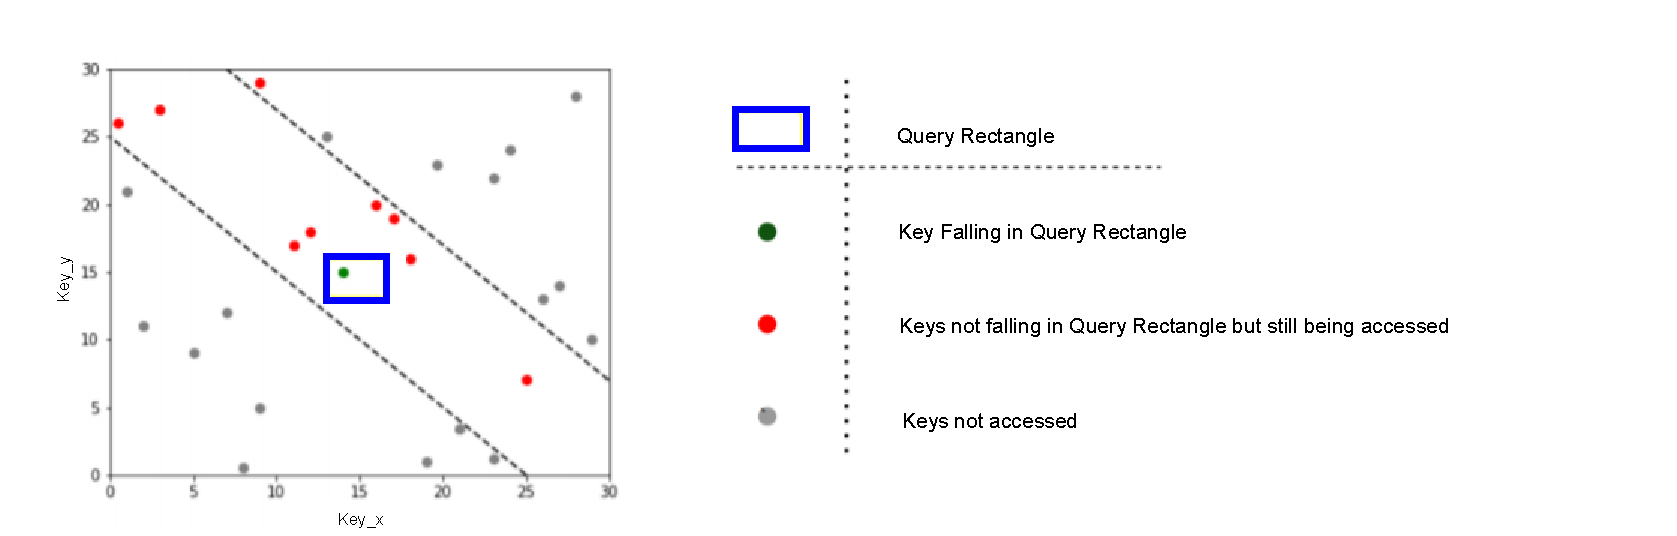
\includegraphics[width=1.3\textwidth]{graphs/Baseline_limitation.pdf}
    \caption{Baseline Method Limitation }
    \label{fig:BaseLine_Method_Limitation}
\end{figure*}
}


\subsubsection {LISA Baseline model search optimization for smaller values of N}
%In lisa baseline model, we need to linearly search for the query key in a cell. 
In case of high dimensional key values, key with in a cell can not be searched with mapped value, as a large number of keys can have the same mapped value. However for the 2 dimensional scenario, we can get considerable savings in search cost by replacing sequential scan based on keys values to binary search based on mapped value. As in the original method, search process  will consist of two parts.
\begin{enumerate}
	\item Find the cell which contains the query key based on mapped value using binary search. 
	\item With in the cell, replace sequential search based on query key value with the  binary search based on query key mapped value. Once mapped value is found, do a lookup in the neighbourhood of the found key based on query key 2 dimensional value. 
\end{enumerate}
As shown in Fig. \ref{fig:LISA_Baseline_Optimization}, we get significant savings in the query time with this approach for smaller values of N. As the value of $N$ increases, number of Keys per cell decreases, and savings in avoiding sequential search gets normalized. 


\begin{figure}
 \centering
     \begin{subfigure}[b]{0.45\textwidth}
         \centering
         \begin{tikzpicture}[font=\small]
	\pgfplotsset{compat=1.10, width=\textwidth, height=\textwidth,every axis
	legend/.append style={
		at={(1,1)},
		anchor=north east}}
	\begin{axis}[
		xmode=log,
		xlabel=$N$,
		ylabel=Average Query Time (ms),
		xtick={10,100,1000,10000},
		legend style={nodes={scale=0.55, transform shape}}
	]
	\addplot[smooth, mark=x, blue]
	coordinates{
		(10, 46.7173)
		(100, 4.8086)
		(1000, 0.7271)
		(10000,0.3301)
		%(100000,0.2381)
	};
	\addplot[smooth,mark=o,red]
  	coordinates{
        (10, 0.2855)
		(100,0.2823)
		(1000, 0.2806)
		(10000,0.2794)
		%(100000,0.2322)
	};
  
    %\legend{LISA Baseline, LISA Baseline Optimized}
	\end{axis}
\end{tikzpicture}
         \caption{Training Size 100K}
         \label{fig:2d_exp4_3_1}
     \end{subfigure}
     \begin{subfigure}[b]{0.45\textwidth}
         \centering
         \begin{tikzpicture}[font=\small]
	\pgfplotsset{compat=1.10, width=\textwidth, height=\textwidth,every axis
	legend/.append style={
		at={(1,1)},
		anchor=north east}}
	\begin{axis}[
		xmode=log,
		xlabel=$N$,
		ylabel=Average Query Time (ms),
		xtick={10,100,1000,10000},
		legend style={nodes={scale=0.75, transform shape}},
		scaled y ticks = base 10:-2,
	]
	\addplot[smooth, mark=x, blue]
	coordinates{
		(10, 347.5613)
		(100, 40.1451)
		(1000, 4.4732)
		(10000,0.6697)
		%(100000,0.2944)
	};
	\addplot[smooth,mark=o,red]
  	coordinates{
        (10, 0.2905)
		(100,0.2858)
		(1000, 0.2844)
		(10000,0.2831)
		%(100000,0.2322)
	};
  
    \legend{LISA Baseline, LISA Baseline Optimized}
	\end{axis}
\end{tikzpicture}
         \caption{Training Size 1M}
         \label{fig:2d_exp4_3_2}
     \end{subfigure}
     \caption{Point query results comparison between LISA Baseline and Optimized Model for different training sizes.}
     \label{fig:LISA_Baseline_Optimization}
\end{figure}



\chapter{Convolution and CNN for Learned Indexes}

$K$-Nearest Neighbours ($K$NN), as the name suggests, is the process of finding $K$ nearest neighbours to a given query point. In this project, $K$NN query is only performed on $2$-dimensional data. We use $\ell_2$ norm as the distance metric. A $K$NN query will be formalised as $\mathcal{K}(\boldsymbol{X})$ where $\boldsymbol{X}\in\mathbb{R}^2$.

\subsubsection{$K$NN query with $K$D-Tree}
As a baseline, we first perform $K$NN query with $K$D-tree.\\
The main advantage of $K$D-Tree is that we can exploit the tree structure and prune points we don't think will have distance smaller than the ones we have already calculated. This improves the time complexity as compared to finding the distance of point with every other point in space to get the closest neighbours. 


\begin{algorithm}[H]
    \SetAlgoLined
    \SetKwInOut{Input}{Input}
    \SetKwInOut{Output}{Output}
    \Input{$K$; \texttt{Number of nearest neighbour, List of TestPoints; $\mathcal{P}(\boldsymbol{x}, \boldsymbol{y}); [x \in \mathbb{R};y \in \mathbb{R}]$}}
    \Output{\texttt{List of $K$ nearest points(ResultList)}}
    \For{$i\gets0$ \KwTo $len(TestPoints)$}
    {
        \texttt{Start at root}\\
        \texttt{Traverse subtree where $\mathcal{P}(\boldsymbol{x}, \boldsymbol{y})_i$ can be added.}\\
        \texttt{Find the leaf; Calculate the distance and store it as $\mathcal{D}$}\\
        \eIf{$len(ResultList) < K$}
            {
                \eIf {\texttt{Perpendicular distance of Parent with $\mathcal{P}(\boldsymbol{x}, \boldsymbol{y}) <= \mathcal{D}$}}
                    {
                        \texttt{Go on the other side of subtree} 
                    }
                        {
                            \texttt{Go up another $level$}
                        }
            }
            {
                \texttt{return ResultList}
            }
        
    }
    \caption{$K$NN Query Algorithm for $K$D-Tree}
    \label{$K$NN_Query_Algorithm_$K$D-Tree}
\end{algorithm}

In algorithm \ref{$K$NN_Query_Algorithm_$K$D-Tree},
\begin{enumerate}
    \item Start with the root to traverse tree until we reach the leaf. We find the subtree where the new $\mathcal{P}(\boldsymbol{x}, \boldsymbol{y})$ could be added and finally reach the leaf of this subtree. 

    \item Calculate the square of the euclidean distance of this point from the $\mathcal{P}(\boldsymbol{x}, \boldsymbol{y})$. We add it to the list and push and pop values from the list depending on the distances we calculate while traversing the tree upwards from here.
    
    \item From the leaf we could either go up another level or go the other side of the subtree to get a point that could have a distance smaller than the last best calculated distance in the list. 
    
    \item Once we make a decision in the above step, we can recursively traverse the tree upwards until we reach the root. 
\end{enumerate}


\begin{mscexample}


    \begin{minipage}[t]{\linewidth}
        \centering
        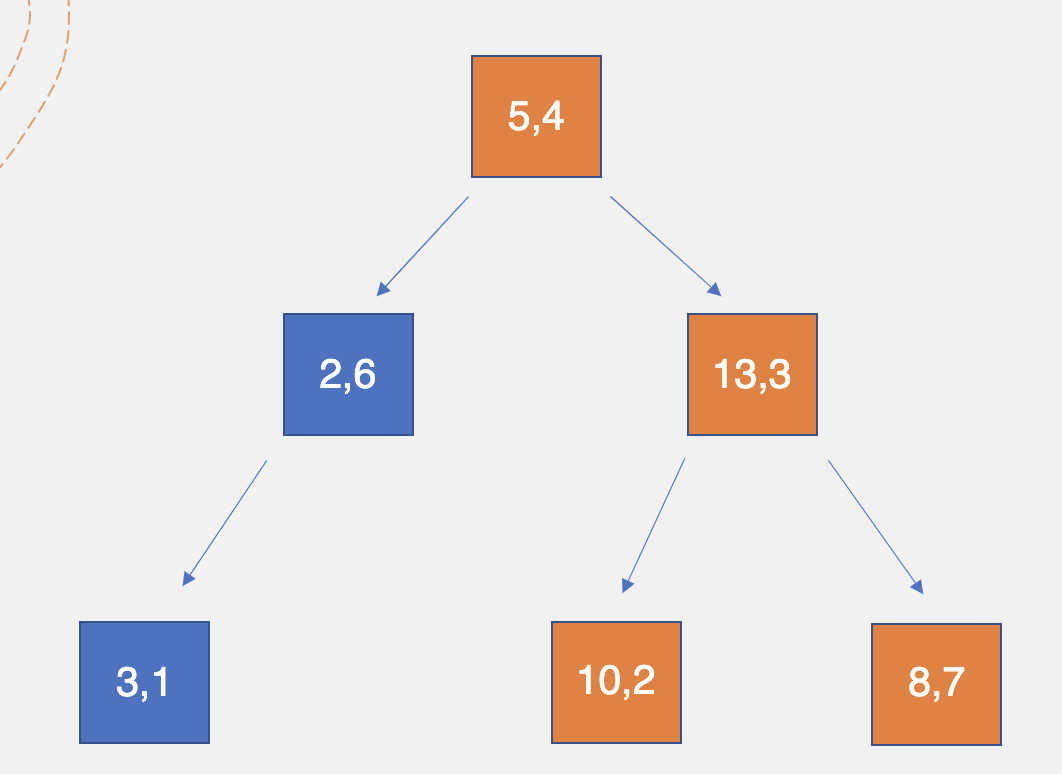
\includegraphics[width=6cm]{graphs/KD-Tree_KNN_Tree.png}
        % \caption{$K$D-Tree for KNN Query}
        \label{fig:$K$D-Tree_for_KNN Query}
        \hfill
        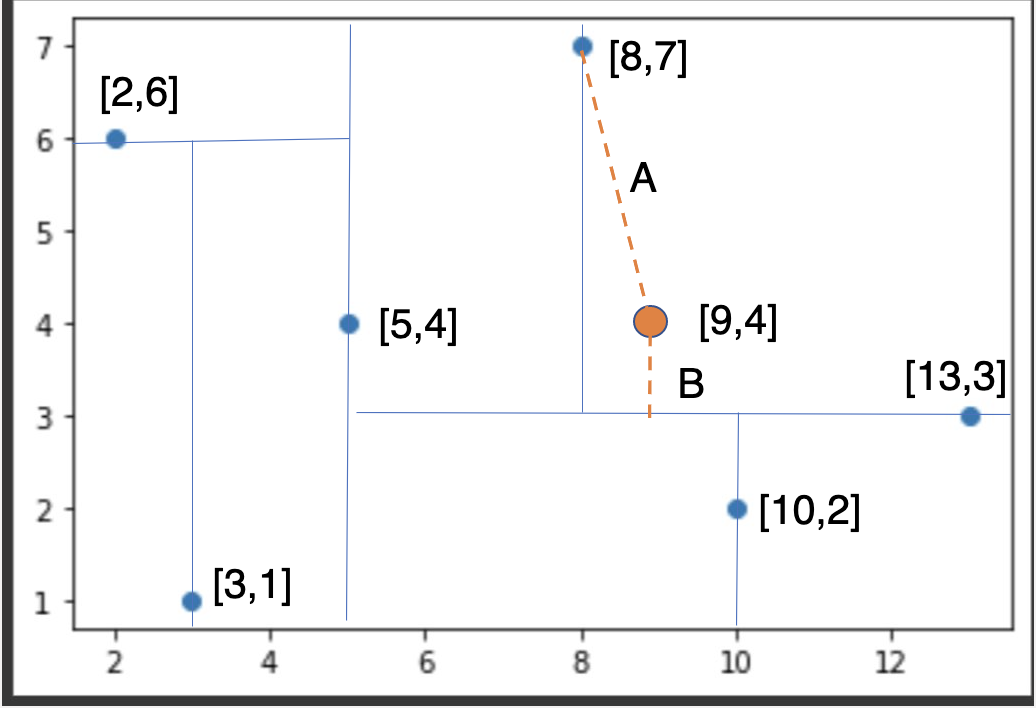
\includegraphics[width=6cm]{graphs/KD-Tree_KNN_plot.png}
        % \caption{$K$D-Tree KNN Plot on 2-dimentional plane}
        \label{fig:KD_Tree_KNN_Plot}
    \end{minipage}
	For example, we have Point list as $$((5,4),(2,6),(13,3),(8,7),(3,1),(10,2))]$$ 
	
	\textbf{Test point; $\mathcal{P}(\boldsymbol{x}, \boldsymbol{y})$} = $(9,4)$\\
	
% 	we will have a tree structure as shown in \ref{fig:$K$D-Tree_for_KNN Query} and it's plot on $2$-dimensional plane is shown in \ref{fig:KD_Tree_KNN_Plot}. *****\ref{fig:KD_Tree_KNN_Plot} \\
% 	In the fig above, we can see that although point $(8,7)$ is the leaf we will reach when we traverse the tree to search where test point $(9,4)$ can be added, it is not in fact the nearest point to the test point. \\
	
	Below are the steps followed to get the $4$ nearest neighbours:
	\begin{enumerate}
    	\item Traverse to $(8,7)$ by searching for a location where $\mathcal{P}(\boldsymbol{x}, \boldsymbol{y})$ could be added.
    	
    	\item Add $(8,7)$ to result list.
    	
    	\item Calculate the distance of $(8,7)$ and $\mathcal{P}(\boldsymbol{x}, \boldsymbol{y})$. Save the distance as $\mathcal{D}$
    	
    	\item Make a decision whether to traverse to the other side of the subtree to point $(10,2)$ by checking the perpendicular distance of $(13,3)$ with $\mathcal{P}(\boldsymbol{x}, \boldsymbol{y})$ and compare this with $\mathcal{D}$.(We do this to verify if there is even a possibility to find a point smaller than the last best distance on the other side of the subtree.) 
    	
    	\item Since the perpendicular distance is smaller than the best calculated $\mathcal{D}$ ($A > B$), we will check the distance of $\mathcal{P}(\boldsymbol{x}, \boldsymbol{y})$ and $(10,2)$. This distance in our case is indeed smaller than the best calculated distance of $\mathcal{P}(\boldsymbol{x}, \boldsymbol{y})$ with $(8,7)$ so far.
    	
    	\item Add $(10,2)$ to result list.
    	
    	\item Similarly, we traverse until we have $4$ nearest neighbour to $\mathcal{P}(\boldsymbol{x}, \boldsymbol{y})$ in the list.
	\end{enumerate}
\end{mscexample}



\subsubsection{$K$NN Query with LISA}
%TODO: What does this paragraph mean?
%We do not know the analytical representation of shards, as we use machine learning model $ \mathcal{SP}$ to generate shards. Thus, 
It is difficult to apply traditional $K$NN query pruning strategies applicable for $K$D-Trees, to LISA model as it doesn't maintain a tree like structure with all nodes and
entries based on MBRs (minimum bounding rectangle) and parent-children relationships. Shard boundaries are learned per mapped interval and no data structure is maintained to refer to shards in adjacent mapped intervals. The key idea in the $K$NN query is to convert it into a range query by estimating an appropriate query range. LISA paper suggests a learning model to learn an appropriate distance bound from underlying training data for every query point and specific value of K. However, we used empirically estimates to learn this distance bound for different values of $K$. This distance bound is used to convert the $K$NN query to range query.The query range is augmented if less than K neighbors are found in a range query. 

Consider a query point $q_{knn}=(x_{0},x_{1})$, let $x^{'} \in V$ be the $K$th nearest key to $x$ in database at a distance value $\delta = \| x^{'}-q_{knn}\|_{2} $. Lets define $ \mathcal{Q}(q_{knn},\delta) \triangleq [x_{0}-\delta, x_{0}+\delta) \times[x_{1}-\delta, x_{1}+\delta)$ and $\mathcal{B}(q_{knn}, \delta)  \triangleq \{p \in V \mid \| q_{knn}-p\|_{2} \leq \delta \} $. We can create a query rectangle $qr =  \mathcal{Q}(q_{knn}, \delta + \epsilon)$ where $\epsilon \rightarrow 0$. As shown in Fig. \ref{fig:KNN_Query_Lisa}, K nearest keys to $q_{knn}$ are all in $\mathcal{B}(q_{knn}, \delta)$ and thus in $\mathcal{Q}$. $K$NN query can be solved using the range query if we can estimate an appropriate distance bound $\delta$ for every query point.

\begin{figure*}[t]
    \centering
    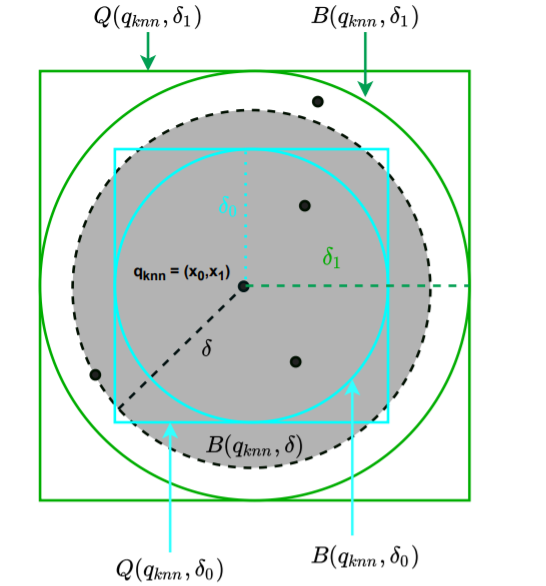
\includegraphics[width=0.7\textwidth]{graphs/KNN_Query_Lisa.png}
    \caption{KNN Query Implementation in Lisa(K=3)\\
    1)$q_{knn}$ represents the query point, $ \mathcal{Q}(x,\delta) \triangleq [x_{0}-\delta, x_{0}+\delta) \times[x_{1}-\delta, x_{1}+\delta)$, represents query rectangle and $ \mathcal{B}(x, \delta)$ represents the key space at distance $\delta$ containing K nearest keys.\\
    2)KNN query can be solved by range query if we can estimate an appropriate distance bound $\delta$ for every query point\\
    }
    \label{fig:KNN_Query_Lisa}
\end{figure*}
In our experiments, we find the $\delta$ empirically. We try with different values of $\delta$ and choose the one for which we get the best results. 

\chapter{Conclusion}

\section*{Acknowledgement}

We would like to express our sincere gratitude to Prof. Dr. Michael Böhlen, and Mr. Qing Chen for their commitment in supervising this project. Our appreciation extends to Dr. Sven Helmer in reading our report and arranging discussion and presentation of this project.

\begin{appendices}
\chapter{Appendix}
\end{appendices}

\begingroup
\fontsize{8pt}{10pt}\selectfont
\begin{landscape}
\begin{table}[]
\footnotesize
\begin{tabular}{|c|c|c|c|c|l|l|l|l|}
\hline
\textbf{\# id} & \textbf{Distributions} & \textbf{root model} & \textbf{second model} & \textbf{third models} & \multicolumn{1}{c|}{\textbf{Build Time (s)}} & \multicolumn{1}{c|}{\textbf{Query Time (ms)}} & \multicolumn{1}{c|}{\textbf{Evaluation   Error (MSE)}} & \multicolumn{1}{c|}{\textbf{Memory Size   (KB)}} \\ \hline
\multicolumn{1}{|l|}{1} &  & fcn & 200 fcn & 2000 fcn & 418.9493798 & 0.970932583 & 653.8536667 & 7487.059896 \\ \cline{1-1} \cline{3-9} 
\multicolumn{1}{|l|}{2} &  & fcn & 200 fcn & 4000 fcn & 1141.521194 & 0.9675528 & \textbf{1.134166667} & 24440.75523 \\ \cline{1-1} \cline{3-9} 
\multicolumn{1}{|l|}{3} &  & fcn & 200 fcn & 6000 fcn & 688.8004486 & 1.07512705 & 196.9116667 & 13034.22656 \\ \cline{1-1} \cline{3-9} 
\multicolumn{1}{|l|}{4} &  & fcn & 400 fcn & 2000 fcn & 483.1734781 & 1.158343717 & 113246.196 & 9208.992183 \\ \cline{1-1} \cline{3-9} 
\multicolumn{1}{|l|}{5} &  & fcn & 400 fcn & 4000 fcn & 636.8463397 & 1.339095933 & 113652.3212 & 12695.55731 \\ \cline{1-1} \cline{3-9} 
\multicolumn{1}{|l|}{6} &  & fcn & 400 fcn & 6000 fcn & 742.0712694 & 1.243333667 & 51.00183333 & 15434.78905 \\ \cline{1-1} \cline{3-9} 
\multicolumn{1}{|l|}{7} &  & fcn & 600 fcn & 2000 fcn & 504.959355 & 1.06512235 & 113246.2647 & 9745.335942 \\ \cline{1-1} \cline{3-9} 
\multicolumn{1}{|l|}{8} &  & fcn & 600 fcn & 4000 fcn & 879.6010201 & 0.973031833 & 18.99766667 & 20434.90626 \\ \cline{1-1} \cline{3-9} 
\multicolumn{1}{|l|}{9} &  & fcn & 600 fcn & 6000 fcn & 373.6126809 & 1.11725315 & 142041.6877 & 8118.023442 \\ \cline{1-1} \cline{3-9} 
\multicolumn{1}{|l|}{10} &  & lr & 200 lr & 2000 lr & 262.5089284 & 1.280502367 & 8246.633985 & 4348.463542 \\ \cline{1-1} \cline{3-9} 
\multicolumn{1}{|l|}{11} &  & lr & 200 lr & 4000 lr & 869.7494701 & 1.304096217 & 7326.238372 & 18769.81252 \\ \cline{1-1} \cline{3-9} 
\multicolumn{1}{|l|}{12} &  & lr & 200 lr & 6000 lr & 655.0431077 & 1.318176683 & 6276.09111 & 13297.72135 \\ \cline{1-1} \cline{3-9} 
\multicolumn{1}{|l|}{13} &  & lr & 400 lr & 2000 lr & 275.3925674 & 1.31789575 & 120427.9247 & 5143.059892 \\ \cline{1-1} \cline{3-9} 
\multicolumn{1}{|l|}{14} &  & lr & 400 lr & 4000 lr & 601.7362665 & 1.453903583 & 6783.428749 & 12864.80731 \\ \cline{1-1} \cline{3-9} 
\multicolumn{1}{|l|}{15} &  & lr & 400 lr & 6000 lr & 388.5866734 & 1.623972083 & 5998.720313 & 8041.416654 \\ \cline{1-1} \cline{3-9} 
\multicolumn{1}{|l|}{16} &  & lr & 600 lr & 2000 lr & 267.8966881 & 1.861582733 & 121932.5051 & 4986.927088 \\ \cline{1-1} \cline{3-9} 
\multicolumn{1}{|l|}{17} &  & lr & 600 lr & 4000 lr & 558.531068 & 1.52717965 & 8434.091306 & 13843.60678 \\ \cline{1-1} \cline{3-9} 
\multicolumn{1}{|l|}{18} &  & lr & 600 lr & 6000 lr & 337.0881814 & 1.28034995 & 35342.6365 & 8366.570317 \\ \cline{1-1} \cline{3-9} 
\multicolumn{1}{|l|}{19} &  & lr & 200 lr & 4000 fcn & 34.86059083 & 1.63086885 & 14478.05283 & \textbf{220.4973958} \\ \cline{1-1} \cline{3-9} 
\multicolumn{1}{|l|}{20} &  & lr & 200 fcn & 4000 fcn & 410.2378013 & 1.653916983 & 13656.1507 & 9318.697933 \\ \cline{1-1} \cline{3-9} 
\multicolumn{1}{|l|}{21} &  & fcn & 200 fcn & 4000 lr & 38.131223 & 1.667702583 & 12191.8397 & 602.2005208 \\ \cline{1-1} \cline{3-9} 
\multicolumn{1}{|l|}{22} &  & fcn & 200 lr & 4000 lr & 238.9569197 & 1.663567483 & 13403.64758 & 5229.914058 \\ \cline{1-1} \cline{3-9} 
\multicolumn{1}{|l|}{23} &  & lr & 200 fcn & 4000 lr & 290.6430138 & 1.657428583 & 12567.93278 & 6588.58335 \\ \cline{1-1} \cline{3-9} 
\multicolumn{1}{|l|}{24} & \multirow{-24}{*}{log\_normal} & fcn & 200 lr & 4000 fcn & 352.6849412 & 1.909310833 & 11572.93555 & 8292.059883 \\ \hline
\end{tabular}
\label{appendix_1: experiments summary of small lognormal}
\caption{}
\end{table}
\end{landscape}
\endgroup


\bibliographystyle{alpha}
\bibliography{refs}

\end{document}
